\documentclass[a4paper,12pt,showkeys]{jreport}
\usepackage{graduatethesis}
\usepackage{listings,jlisting}
\usepackage{pifont}
\usepackage{cite}
\pagestyle{plain}

\makeatletter
%\def\@cite#1{$\m@th^{\hbox{\@ove@rcfont #1)}}$}
\makeatother

\title{シナリオ・ツリー型モデルを利用した\\風力発電設備の安定運用計画の立案}
\author{シス05-19 臼木 誠}
\date{\today}
\西暦

\begin{document}
\maketitle
\setcounter{tocdepth}{2}

\pagenumbering{roman}
\tableofcontents
\newpage
\pagenumbering{arabic}

\chapter{はじめに}

日本では,東北地方太平洋沖地震での福島第一原子力発電所の事故によって原子力発電の危険性が再認識され,
原子力発電所の見直しや稼働停止などがはじまった.
そして,原子力に変わる安全性のある新たなエネルギーとして,再生可能エネルギーが今まで以上に目が向けられるようになってきた.

再生可能エネルギーとは,自然環境の中で繰り返し起こる現象から取り出すエネルギーの総称である.
再生可能エネルギーは,二酸化炭素等の温暖化ガスの排出量が少ないものが多いことから低炭素社会への貢献にもつながり,
普及拡大に向けて世界で導入が広く検討されている.
しかし,再生可能エネルギーの発電ではまだ課題などが多く,原子力発電のような安定した電力の供給は難しい.

本研究室で前年度からテーマとして取り上げている風力発電も再生可能エネルギー発電の一つであり,実用化が進められているが,
様々な問題を抱えている.
例えば,騒音や低周波といった人にとっての環境問題や鳥類の衝突事故(バードストライク)などの問題を抱えているが,
諸問題の中でも,出力変動や強風対策などの技術的課題が風力発電の運用を困難にしている.
風力発電は欧米での開発や研究が進んでいたが,近年は日本の企業や研究機関による日本の風況に適した風車の開発も活発に行われている.

そこで本研究では,風力発電の出力変動を抑え,安定した電力の供給を行い,事業の利益も追求することを目的とした研究を行う.
前年度の卒業研究\cite{徳谷}では風を不完全情報として扱い,オンラインアルゴリズム的思考に基づいた運用計画の立案を行った.
本研究では,気象庁の過去の風況データを用いて,風速がどのようなパターンで変化するかの確率評価を行い,シナリオ・ツリー型モデルを
考慮した運用計画を立案する.

\newpage
\chapter{風力発電}
\section{WF(ウィンドファーム)の発電,送電}

風力発電は,風の力で風車のブレード(回転羽根)を回し,発電機を使って,回転運動エネルギーを,電気エネルギーに変換するシステムである.
風力発電機のブレードが回転することによって回転軸が回り,発電機を動かし発電する.
回転軸と発電機の間には増速機(歯車)があり,ゆっくりとしたブレードの回転を,発電機が必要とする回転速度まで高める役割をする.
他には風が強い場合に少し羽根をねかせて風圧を調整する可変ピッチ機構,風力発電機が正しく風の方向を向いて最も効率的な発電が
行えるように風力発電機の方向を制御する方向制御機構などが備わっている.
また,台風や突風などの強風対策にブレーキ装置も取り付けられており,カットアウト風速を超えると,ブレードを停止させることもできる.
風力発電量は,受風面積と風速の3乗に比例する.
よって,発電量は面積と空気密度が同じと考えるなら,風速の3乗に比例して強くなる \cite{牛山}.
例えば,風速が2倍になれば,8倍の発電量を得ることができる.しかし,逆に風速が1/2倍になれば発電量は1/8倍になるので,発電量の変動が非常に激しい.
そこで風力発電の早くて激しい出力変動を抑えるために蓄電池を設置し,蓄電システムの充放電によって総合出力を平滑化し,
電力系統に送電している.
送電された電力は,電力会社(系統)に購入される.
電力の購入価格は,昼夜間によって価格が違い,需要の高い昼間は高く,需要の低い夜間は安くなっている.
電力の単価は電気価値分が3~4(円/kWh),環境付加価値が6~7(円/kWh)で構成されており,合成単価で大体9~11(円/kWh)となっている.
風力は再生可能エネルギーのひとつとして,地球環境の保全,エネルギーセキュリティの確保可能なエネルギー源として認められ,
開発可能な量だけで人類全体の電力需要を充分に賄える資源量があるとされる.

以下に,風力発電のメリット・デメリットを挙げる.
\begin{itemize}
\item メリット

主に環境負荷の小ささ,化石燃料の使用量削減,エネルギー安全保障などが挙げられる.

\begin{itemize}
\item 発電時に地球温暖化の原因となる二酸化炭素等の温室効果ガスを排出しない.

\item 比較的発電コストが低く,事業化が比較的容易である.

\item 太陽光とは違い,風が吹けば24時間発電可能である.

\item エネルギー自給率の向上が見込める.

\item 冷却水を必要としない.
\end{itemize}
\end{itemize}

\begin{itemize}
\item デメリット

主に出力電力の不安定・不確実性と,周辺の環境への悪影響の問題があり,特に設置場所の選定が重要となっている.
\begin{itemize}

\item 風速の変動に伴い,出力される電圧などが需要と関係なく変動してしまう.

\item 風力発電機を設置する場所の風況が発電の採算性に大きく影響する.

\item 風車などの発電機のブレードにワシやタカなどの希少猛禽類の幼鳥が衝突(バードストライク)して死亡するケースがある.

\item 周囲に騒音被害や,低周波による人体への悪影響がある.

\item 観光地に風力発電機を設置する事で景観への影響がある.
\end{itemize}
\end{itemize}

\section{風車の種類}

風車の回転軸の方向で分類すると水平軸(主にプロペラ)型と垂直軸型の二つに大別される.
また,風車のトルク発生形態からみると,風車の翼に
生じる抗力を利用するものと,揚力を利用する形式とに分類できる.
風力発電には主に揚力形の風車を利用する.
以下に代表的な風車を紹介する\cite{牛山}.
\begin{quotation}
\begin{itemize}
\item 水平軸型風車

\begin{itemize}
\item プロペラ型風車

\begin{figure}[h]
\centering
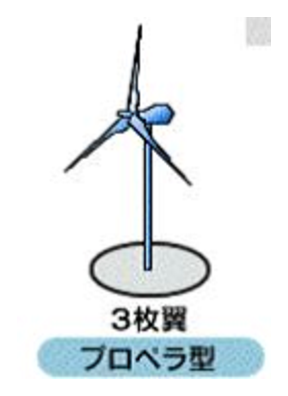
\includegraphics[width=2cm, clip]{fuusya1.eps}
\caption{プロペラ型風車}
\label{fig:fuusya2}
\end{figure}

プロペラ型は,羽根の回転軸が水平になっており,ブレードは飛行機のプロペラと同じ断面をもっていて高速回転する.
現在,実用化されている風力発電の中で最も普及しているのがこの型となる.
プロペラ型は発電効率が良く,低風速でも自己起動が可能で,大型化が容易なので,大きな電力の発電も可能である.
しかし,発電機などの重量物も風車上部に取り付けなければならないという設置・メンテナンス時の操作性の問題と,
風車の回転面を常に風の方向に向ける必要があるという問題がある.
また,高速回転に優れた特性を持っているが,反面騒音が大きいという問題も抱えている.
基本的には3枚羽根の風車が多いが,流体力学的には風車の翼数が
少ないほど高速回転するとされ,中には高速に回転させるため1枚羽根や2枚羽根の風車も存在する\cite{設備}.
\end{itemize}
\end{itemize}


\begin{itemize}
\item 垂直軸型風車

\begin{itemize}
\item サボニウス型風車

\begin{figure}[h]
\centering
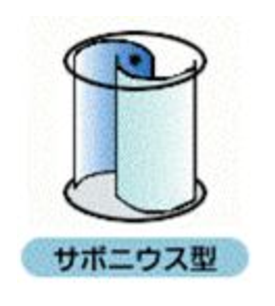
\includegraphics[width=2cm, clip]{fuusya2.eps}
\caption{サボニウス型風車}
\label{fig:fuusya2}
\end{figure}

駆動部を垂直軸にすることで,風向に影響されることなく,駆動部を回転させて発電することができる.
風車の回転力(駆動トルク)を主として作動要素の空気抵抗で得るものを抗力型風車と呼んでおり,風車構成要素の凸側と凹型の抵抗が
異なっていることを利用して風による風車要素を押す力(抗力)により回転力を得ている.
風を切らない構造の為,静寂性に優れ都心部など風向きが変わりやすく,騒音に配慮しなければならない条件の場所でも効率良く配置することができる.
また発電機が地上近くにあることからメンテナンス性も良い.
しかし,発電効率はあまり高くなく,小型な風車が主体であり,1台あたりの出力は小さい\cite{設備}.
関西大学凛風館の屋上に設置されている風車は,このサボニウス型風車である.

\item ダリウス型風車

\begin{figure}[h]
\centering
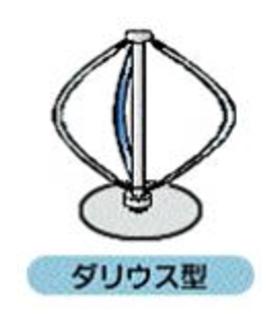
\includegraphics[width=2cm, clip]{fuusya3.eps}
\caption{ダリウス型風車}
\label{fig:fuusya2}
\end{figure}

縦方向に湾曲して伸びる羽根が風を捕捉し,回転し発電する.風車構成要素から発生する揚力を主に利用して回転力を得るものを揚力型風車
といい,飛行機の翼に用いられるような断面形状をした風車構成要素を用いている.
サボニウス型にも言えるが,コストの低さ,騒音の無さ,風向制御機構が不要なことから,都心部などに設置しやすい.
しかし,プロペラ型風車より発電効率が低く,発電量の確保が困難なことから,発電設備としてではなく,デザイン的な観点やアピール用としての利用が主体となる\cite{設備}.

\end{itemize}
\end{itemize}
\end{quotation}

\section{制御型}

本節では,風力発電の制御型について説明する,制御型には出力一定制御型と出力変動緩和型の2通りがある.
ここでは,まず2通りの制御型の共通事項について説明し,その後に個別の制御型について述べる.
最後に制御型の技術要件に関する課題について述べる.


\subsection{出力一定制御型と出力変動緩和型に関する共通事項}

以下は東北電力\cite{風力}による出力一定制御型と出力変動緩和型に関する共通事項である.

\begin{itemize}
\item 周波数変動対策として蓄電池を設置し,蓄電池出力を制御することによって,風力発電に起因する出力変動をほぼ皆無とすること.

\item 蓄電池との組み合わせによる風力発電の計画的な運転,送電の可能性を検証するため,当社に事前に連絡する発電計画に基づく運転を行うこと.

\item 平時は,周波数変動対策後の風力発電設備合成出力(1分間平均値)と発電計画に基づいて決定される制御目標値との偏差を,
周波数変動対策後の風力発電設備合成出力の最大出力の$2\%$以下とすること.

\item 周波数変動対策後の風力発電設備合成出力を,発電計画に基づき変更する場合の制御については,1分あたりの合成出力の変化を,
周波数変動対策後の風力発電合成出力の最大出力の$2\%$以下とする.ただし,電力を購入する者が,発電計画を指定する場合は,当社,
電力を購入する者,および,風力発電事業者の協議によって定めるものとする.

\end{itemize}
\subsection{出力一定制御型}

出力一定制御型では,風力発電に蓄電池を併設し,蓄電池の充放電制御により,風力発電出力を一定に制御し,計画的に発電する.
事前に電力目標値(kW)と電力量目標値(kWh)を通告する必要があり,発電出力は目標値の$\pm2\%$以内を一定とする\cite{出力一定}.

\begin{figure}[h]
\centering
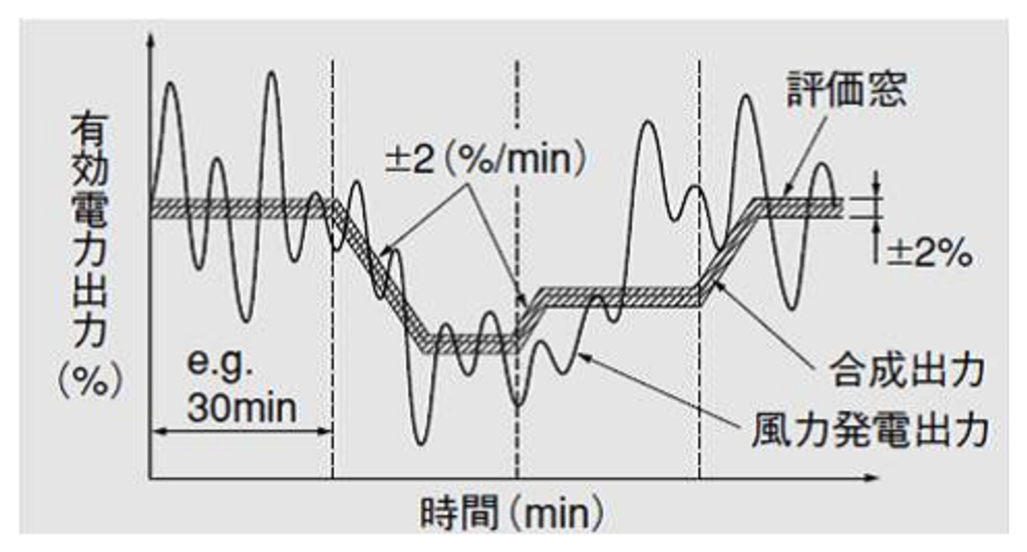
\includegraphics[width=9cm,height=5cm, clip]{seigyo1.eps}
\caption{出力一定制御型\cite{風力}}
\label{fig:seigyo1}
\end{figure}

出力一定制御型は,数時間先から2~3日以降の風力発電出力の予測情報を元に,事前に運転計画を立て,電力会社に通告する必要がある.
通告運転をする際,予測された風力発電出力には誤差を含んでいるため,実際の運転においては,この誤差を考慮しながら蓄電池の制御を行なうこととなる.
蓄電池の容量が大きければ大きいほど,事前の通告通りに合成出力を制御することが容易になり,逸脱率も縮小される.
しかし,風力発電設備が大規模になるほど要求される蓄電池も巨大になるので,事業性を考慮した場合,出来るだけ少ない容量の
蓄電池が望ましい.

技術要件において,発電計画の通告時間や発電計画の変更の可否については明示されていない.
電力系統への反映を考慮すれば,前日の通告と必要に応じた1~2時間前での通告変更が最低限求められる機能であると
考えられる.
併設する蓄電池については充放電可能な容量も限りがあり,発電量予測精度が悪ければ蓄電池の充電状態の管理が困難となり,
蓄電池が満充電状態や完全放電状態に到達してしまうと,発電出力を制御できない状態に陥る.
従って,蓄電池の充電状態に応じて逐次発電計画を変更できれば,蓄電池の運用性も向上する.
一定周期での通告変更が可能であれば,予測精度が向上するだけではなく,必要な蓄電池容量を低く抑える効果が期待できる.

出力一定制御型の検討を行う時,滞在率の評価も行う.
滞在率は(技術要件を満たす時間の総和/全運転時間)$\times$$100\%$と定義する.
現状では技術要件の中で滞在率の概念は定義されておらず,平常時には$100\%$の滞在率を達成させることが求められる.
しかし,技術要件を常に$100\%$を達成することは困難であり,$1\%$程度の逸脱ならば許容される\cite{電力}.

\subsection{出力変動緩和型}

出力変動緩和型では,風力発電に蓄電池を併設し,蓄電池の充放電制御により,風力発電の出力変動を緩和する.
出力変動緩和型は,風車の定格出力の変動を変動を緩和することに重点を置いている.

\begin{figure}[h]
\centering
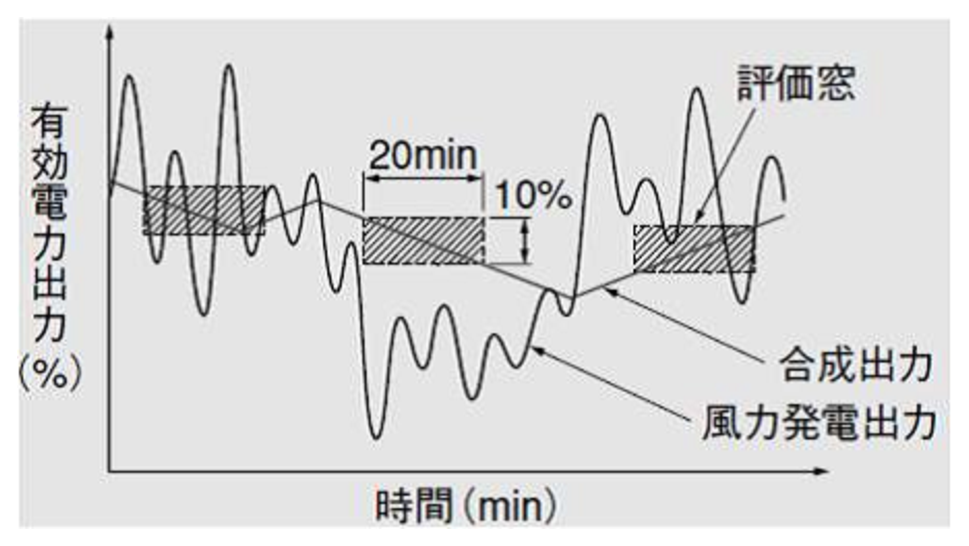
\includegraphics[width=9cm,height=5cm, clip]{seigyo2.eps}
\caption{出力変動緩和型\cite{風力}}
\label{fig:seigyo2}
\end{figure}

平時は,任意の時刻から始まる20分間において,周波数変動対策後の風力発電設備合成出力(1分間平均値)の「最大値\-最小値」が、
風力発電機の定格出力合計値の10\%以下であること.
20分間の変動を10\%に抑制するもので,0[kW]~定格出力まで100\%の出力変化を200分掛けてゆっくりと変化させるものである\cite{変動緩和}.

\subsection{制御型の技術要件に関する課題}

電力系統の電源設備にはそれぞれ役割があり,系統周波数を維持するLFC(Load Frequency Control: 負荷周波数制御)電源と
EDC(Economic Dispatching Control: 経済負荷運用)電源の2種類に大別される.
LFC電源は数分~数十分程度の需給バランスを維持するように運転され,EDC電源は発電出力が一定時間,
一定出力とした運用がされる.
風力発電の出力変動はLFC電源の容量不足の原因となることが指摘されており,いずれの技術要件もLFC電源への影響軽減が
主たる目的である.
出力変動緩和型は発電出力の数分~数十分の変動抑制に主眼を置いており,LFC電源への影響を軽減することが目的である.
また,出力一定制御型では事前に発電計画を通告することが求められており,これが実現すれば,風力発電を連系容量の制約を
受けない発電設備と位置づけられる可能性がある.
さらに,事前に通告した通りに風力発電を運用可能となれば,発電出力の高付加価値化に結びつく効果も期待される\cite{電力}.

\section{蓄電池}
\subsection{蓄電池を設置する理由}

蓄電池併設風力発電システムは,自然エネルギー電源の設置者側に電力系統の安定性を損なわないように一定の責務を求めるものであり,
蓄電池併設による設置費用や導入費用(イニシャルコスト)の増大など,事業の採算性の悪化が危惧されている.

蓄電池を設置する主な理由としては,風力発電の不規則な出力を平滑化するといった出力制御が目的である.
短周期変動成分を蓄電池で吸収することで,風力導入拡大時に必要となるLFC容量を削減することが可能である.
電力会社の電源設備への周波数対策,夜間などの下げ代不足への出力制御などこれらの問題を解決することができる.
蓄電池の利用により計画発電が可能となれば,売電単価の向上や,系統連系容量の制約を受けない発電設備ができるなど,
付加価値を向上する効果も期待できる.
安定した出力制御や付加価値向上効果が期待できれば,市場拡大のきっかけとなる.
市場拡大による大量生産が始まればイニシャルコストは急激に下がると予想されるが,それにはまだ有効な大規模初期需要がない.
蓄電池併設の可能性としては,大規模需要ができれば,蓄電池の有効初期需要になり蓄電池自体の大幅なコストダウンが期待できる.
蓄電池オプションの推進⇒蓄電池オプションの価格競争力アップ⇒風力の競争力拡大⇒風力市場の拡大という
ポジティブスパイラルができる\cite{併設}.

系統安定化のための蓄電池としては,いくつかの特性で従来の鉛蓄電池よりも優れた特徴を示す電池が開発されてきているものの,
系統安定化用の蓄電池として特性・寿命・コスト等の全て要件を満足するためには,蓄電池の得手を伸ばし,
不得手を抑えるシステムの構築に加え,可能性のある蓄電池の系統安定化用途に向けた技術開発も引き続き必要と考えれる\cite{蓄電池}.

\subsection{蓄電池の種類}

風力発電に使われている2種類の蓄電池を以下に紹介する.

\begin{itemize}
\item 鉛電池
\end{itemize}
\begin{quotation}

\begin{figure}[h]
 \begin{minipage}{0.5\hsize}
  \begin{center}
   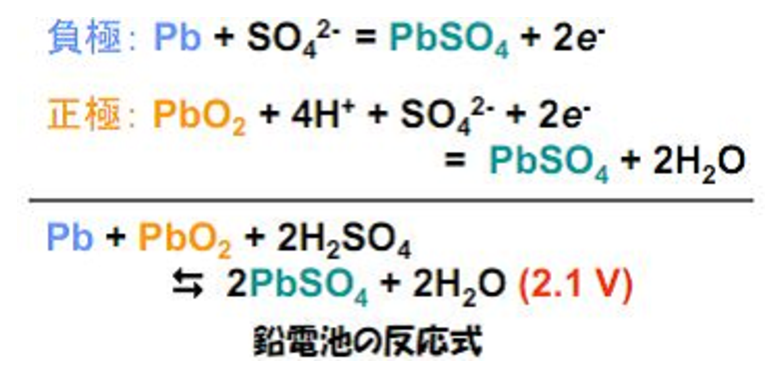
\includegraphics[width=70mm,clip]{namari1.eps}
  \end{center}
  \caption{鉛電池の反応式\cite{蓄電池}}
  \label{fig:one}
 \end{minipage}
 \begin{minipage}{0.5\hsize}
  \begin{center}
   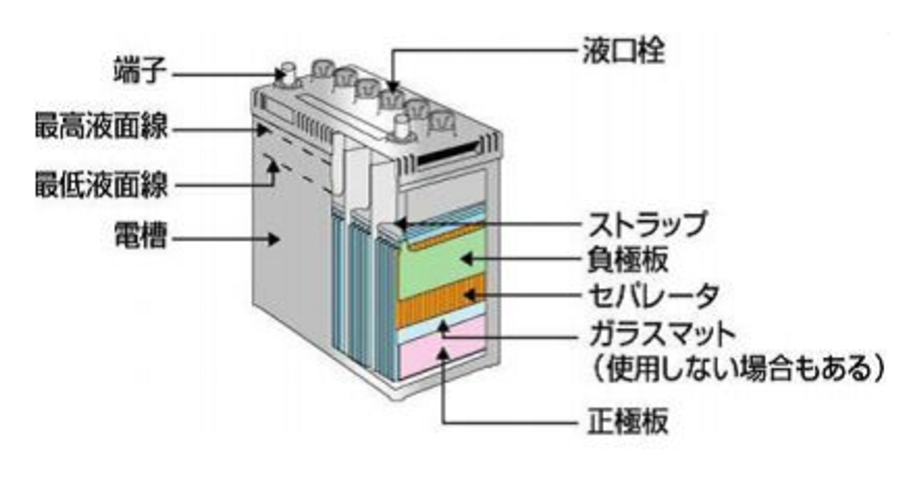
\includegraphics[width=70mm,clip]{namari2.eps}
  \end{center}
  \caption{鉛電池の構造例\cite{蓄電池}}
  \label{fig:two}
 \end{minipage}
\end{figure}


鉛電池は,正極(陽極板)に二酸化鉛,負極(陰極板)には海綿状の鉛,電解液として希硫酸を用いた二次電池である.
他の蓄電池に比べ大型で重く,希硫酸を使うために漏洩や破損時に危険が伴う.
希硫酸の代わりに安全なシリコン液を電解液とするバッテリーもある.
高い電圧を取り出すことができ,電極材料の鉛も安価であることから,二次電池では最も生産量が多い.
使用実績が多く,比較的広い温度範囲で動作し,過充電にも強い.
短時間で大電流放電させたり,長時間緩やかな放電を行なっても比較的安定した性能を持っている.
しかし,低い充電状態では,電極の劣化が進行し充放電サイクル特性に加え,出入力が低下する.
また,充放電エネルギー効率が,他の電池系よりも低く,75~85\%程度である.

放電時に発生する硫酸鉛が結晶化すると,サルフェーションと呼ばれる現象を起こして充放電の容量を著しく低下させる.
サルフェーションとは,極板に硫酸鉛の結晶が付着し,極板が化学反応しなくなる現象である.
開放型バッテリーの極板に白い結晶ができる現象であり,このような状態になるとバッテリー液を補充しても元の状態に回復しなくなる.
バッテリーを長期間使用していると電極板に不活性な硫酸鉛が析出してくるため,バッテリーの通電機能の低下が起こる.
また,寒冷地では比重の低下に伴って電解液が凍結しやすくなり,場合によっては破裂する恐れがあるため,満充電の状態を維持することが望ましい\cite{蓄電池}.

\end{quotation}

\begin{itemize}
\item NAS電池(ナトリウム・硫黄電池)
\end{itemize}
\begin{quotation}

\begin{figure}[h]
 \begin{minipage}{0.5\hsize}
  \begin{center}
   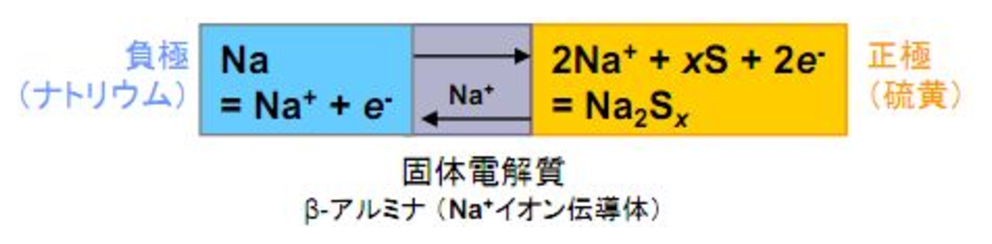
\includegraphics[width=7cm, height=3cm, clip]{nas1.eps}
  \end{center}
  \caption{NAS電池の反応式\cite{蓄電池}}
  \label{fig:one}
 \end{minipage}
 \begin{minipage}{0.5\hsize}
  \begin{center}
   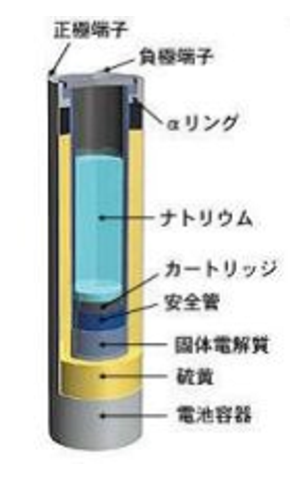
\includegraphics[width=7cm,height=6cm, clip]{nas2.eps}
  \end{center}
  \caption{NAS電池の構造例\cite{蓄電池}}
  \label{fig:two}
 \end{minipage}
\end{figure}

NAS電池とは,負極にナトリウムを,正極に硫黄を,電解質にβ-アルミナを利用した高温作動型二次電池である.
特に大規模の電力貯蔵用に作られ,昼夜の負荷平準などに用いられる.
従来の鉛蓄電池に比べて体積・重量が3分の1程度とコンパクトなため,都市部など需要地の近辺に設置できる.
構成材料が資源的に豊富かつ長寿命,自己放電が少ない,充放電の効率も高い,量産によるコストダウンも期待できるなどの長所も持つ.
しかし,常温では動作しないため,作動温度域(300℃程度)に温度を維持する必要がある.
連続充電・放電時の発熱(電池内部抵抗に基づく)で温度維持されるように設計されており,蓄電システムの利用率が下がると,
温度保持のためヒーター電力が必要である.
充放電特性が比較的長い時間率(6~7時間)で設計されている.また現状では,一定期間に満充電リセットの必要がある.
再生可能エネルギー連系では,商用電力によるリセットの頻度を減らす技術が必要である.

また,風力発電では,満充電状態,完全放電状態になると制御不能になってしまうので,これらの状態にならないように蓄電池の制御管理を
しなければならない\cite{蓄電池}.

\end{quotation}


\section{風速による発電量}

風力発電量の試算方法は,以下の式で計算できる\cite{牛山}.

\[
  P = Cp \times \frac{1}{2} \times \rho \times A \times V^3 \times \eta 
\]

\begin{quotation}
\it$P$[kW]:風力から得られる電力,
\it$Cp$:ベッツの法則からなる電力係数(ベッツ係数),
$\rho$[kg/m$^3$]:空気密度,
\it$A$[m$^2$]:ブレードの受風面積,
\it$V$[m/s]:風速,$\eta$:発電設備の効率
\end{quotation}

この計算式から,風力発電量は受風面積と風速の3乗に比例していることがわかる.
ベッツ係数とは,「風エネルギー」を「運動エネルギー」に変換する際の効率のことをいい,その最大効率が59.3\%であることが証明されている.
これを「ベッツの法則」「ベッツの限界」などと呼んでいる.
しかし,59.3という数字は理論的に導き出された理想上の限界値であり,
実際の風力発電機の風車においては,20~45\%程度のエネルギー変換効率となっている.
発電設備の効率は,風力発電の運転制御,AC-DC変換などのロスから考えると効率は60\%~80\%である.
風車が発電を始める風速は,風速2~3[m/s]からとなる.
充分な発電量を見込みたい場合は,常時風速7.0[m/s]以上の風を得られる環境で発電を行うのがよいとされる.

\section{発電出力予測技術}

蓄電池を併設した風力発電設備において,重要な手法の一つが発電出力予測技術である.
予測システムでは,LOCALS(Local Circulation Assessment and Prediction System)により,12時間ごとに発表される気象予測データである
RSM-GPV(Regional Spectral Model Grid Point Value)を基に予測地点における空間分解能,時間分解能を細分化して,WF内の
各風車における風速・風向データ及び風車の発電出力特性を考慮して,WF全体の発電出力の総和を予測する.
予測データは,10分平均値からなり,最大で48時間分の予測が可能である.
最近では,RSM-GPVに相当するデータは日本域GSM-GPVデータへと変わり,予測時間が84時間まで伸び,1日に4回(3:00,  9:00
, 15:00, 21:00)の発表となっている.
また,21:00発表のデータは192時間先までの予測時間となっている.
さらにWFの風向・風速・発電出力の実績データを元に30分間隔で予測データの更新が行なわれる\cite{電力}.
下図に予測システムとWF間のデータ授受のフロー図を示す.

\begin{figure}[h]
\centering
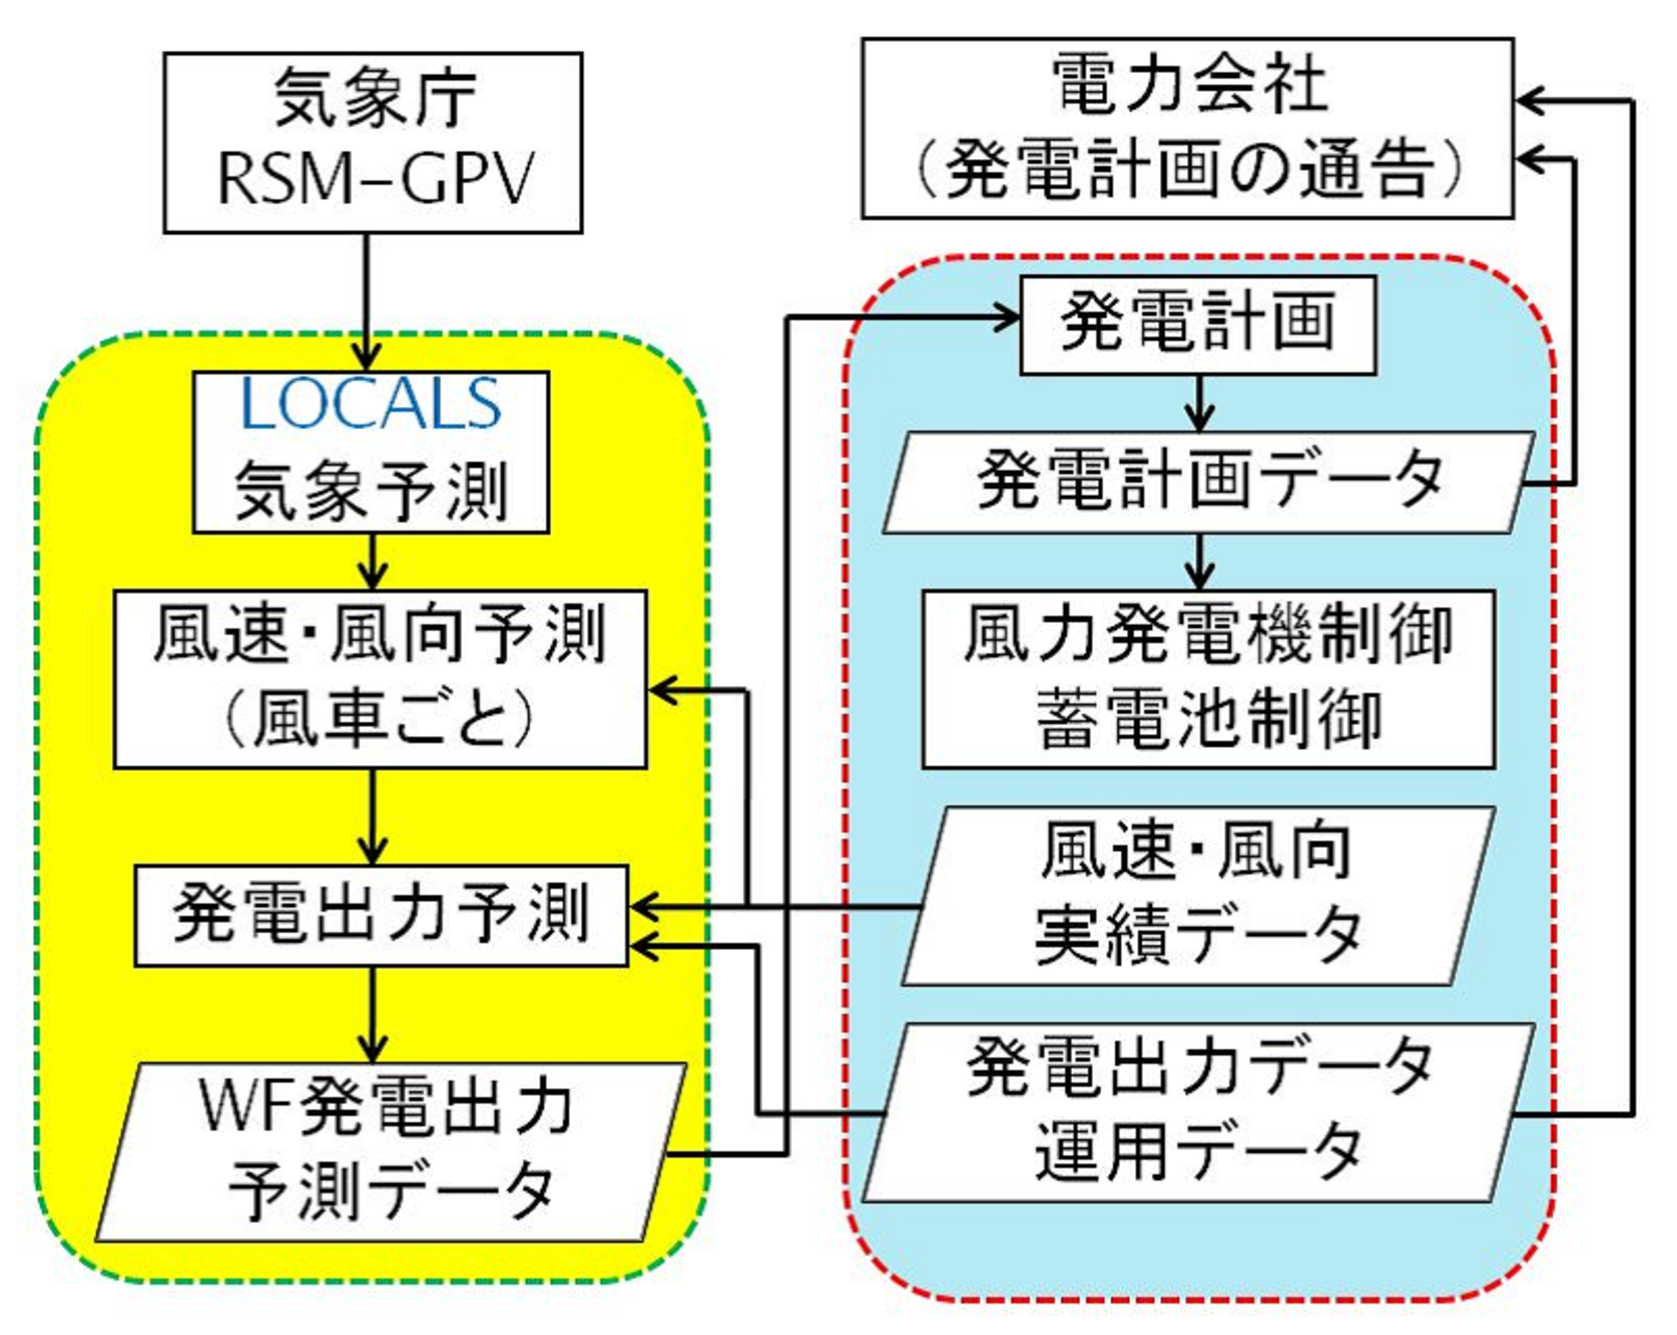
\includegraphics[width=9cm,height=7cm, clip]{yosoku.eps}
\caption{発電出力予測と運用・制御のフロー図\cite{電力}}
\label{fig:yosoku}
\end{figure}

発電予測データの更新には実運用データが必要であり,予測データと実運用データの授受を定期的に行なう.
出力一定制御型において,発電出力予測の手法の精度が良ければ,事前の通告通りに合成出力を制御することが容易になり,
かつ滞在率の逸脱率も縮小される.
また,発電出力予測には翌日予測と当日予測のがあり,この2つを用いて発電計画の決定を行う.
翌日予測は,翌日の30分毎の発電出力を前日の朝に予測し,実際の発電出力の誤差は20\%である.
当日予測は,24時間先までの30分毎の発電出力を30分毎に更新し,こちらの誤差は15\%となっている\cite{予測}.


\section{日本と世界の導入状況,事業}

日本の風力発電設備の導入量は,2010年度末に総設備容量244万kWを超え,総設置基数1814基を達成している.
また,これまでの累計導入量について,設備容量を設置基数で割ってみると,1基当たりの平均設備容量は,
2004年度末から1000(kW/基)を超えており風車の大型化が進んでいる.
地域別にみると,風況に恵まれた北海道,東北,九州地方への設置が大半を占める.
風力発電については,近年,RPS法の施行,系統連携技術要件ガイドラインの整備により,
発電した電力を電力会社に売ることが可能となったため,売電事業を目的とした設置も増えている.
また,風力発電設備の大型化,事業規模の拡大を行うことにより,設置コストや発電コストも大幅に低下させることができる\cite{NEDO}.

日本における今後の風力発電としては,日本の風況にあった風車の開発とこれを安全かつ有効に推進するためのアプリケーション開発が,
これからの日本の市場で要求される.
その内容としては,風の可変性に柔軟に対応できる機能,低い風速でも効率良く発電,移住地域近郊での住民への十分な配慮,
風車の強風時の安全性,充電システムとの連系,鳥獣への安全配慮,環境にやさしい材料の使用,景観を壊さないデザインなどが挙げられる\cite{吉田}.

世界で風力発電の総累積導入量の多い国の順位は中国,アメリカ,ドイツ,スペイン.中国は2004年から6年連続で前年比2倍の成長を遂げ,
2010年にはアメリカを抜いて累計導入量で世界一となる.
新規導入量でも世界の46\%を中国が占める.
世界全体で日本はわずか約1.3\%で13位である.

\begin{figure}[h]
\centering
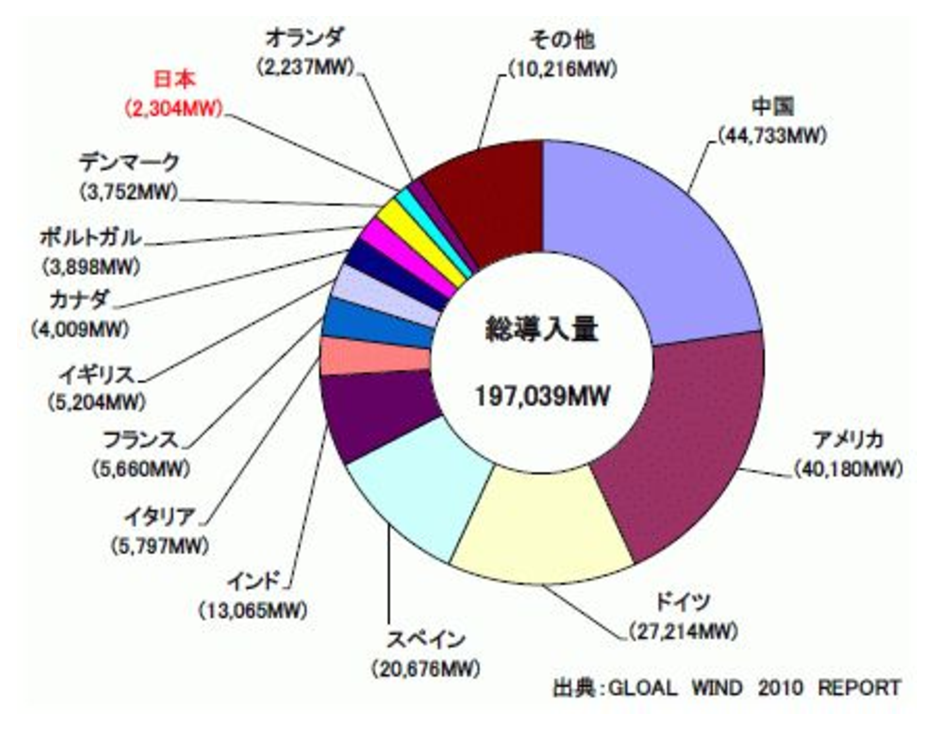
\includegraphics[width=9.5cm,height=6.5cm, clip]{sekai.eps}
\caption{国別風力発電導入割合\cite{エネルギー}}
\label{fig:sekai}
\end{figure}

欧米や中国に比べて日本での風力発電の普及は遅く,日本の風力発電導入量は2011年3月で総設備容量は約245万kWである
(標準的な原発1基の発電量は100万kW前後).
風力発電の設置工事の工期は,1基で約3~4ヶ月と工期が短く,比較的発電コストが安い.
また二酸化炭素の排出削減を見込めることから,日本でも導入が本格化しつつある\cite{エネルギー}.

世界では近年,洋上風力発電の建設が進む.
日本も陸上から立地や輸送の制約のない海上での実証実験がはじまる.
東京電力とNEDOは2010年6月から千葉県銚子沖で洋上風力発電の実証実験を開始した.
実証で使用されるのは,直径約90mの風車を備える風力発電設備1基で,研究期間は2014年3月までとされている.



\chapter{研究目的}

本節では,本研究の目的について述べる.

\section{風力発電設備の安定運用}

最近の風力発電は,その不規則な出力から蓄電池を併設することで安定運用を目指している.
風力発電の安定運用には蓄電池の運用方法が最も重要となってくる.
蓄電池は満充電あるいは完全放電状態になると,出力制御ができなくる.
そこで予測発電量と蓄電池の残存容量を考慮して,蓄電池の充電量ができるだけ50\%に近づくように,
発電計画値に偏りを加える.
このことを蓄電池容量管理という\cite{風力}.
蓄電池は,充放電に伴って充放電効率や補機などのロスが発生してしまう.
これらのロスを考慮して,予測発電量に対して立てる発電計画値を若干下げる必要がある.
売電価格は,昼間は高く,夜間は安くなっている.
この昼夜間の売電価格の差異を利用して,収支を改善することができる.
昼間は,売電価格が高いので蓄電池の放電を多めにして,夜間は売電価格が安いので充電を多めにする.
これらの蓄電池の運用を考慮して,運用計画を立案する必要がある.

\section{前年度の研究とその問題点}

本研究室における前年度の研究\cite{徳谷}では,風力発電の運用に対して,オンラインアルゴリズム的思考に基づいた運用計画を提案した.
オンラインアルゴリズムとは,将来を全く知らない,あるいは不完全情報を考慮した問題を取り扱うためのアルゴリズムである.
オンラインアルゴリズム的思考に基づいた風力発電の運用計画の最悪のシナリオは,運用計画を中断せざるを得ない状況に陥ることであった.
\cite{徳谷}では,そのようなことが生じない,あるいは生じにくい運用計画を立案することにその目標があった.
具体的には,出力一定制御型に対する運用計画を立案するために,出力一定制御型の技術要件,蓄電池の性能や充放電効率,
昼夜間の売電価格の差などをオンラインアルゴリズム的思考に基づき運用計画をモデル化した.

予測発電量と実際の発電量を疑似乱数生成器メルセンヌ・ツイスタを使用し,$64$時間毎に$20$分間隔で予想発電量を決め,
その間の予想発電量は線形補間によって定めた.
これらの要素を用いて$1$日に$72$回送電量を調整し,実験対象期間を30日間とした.
さらに昼間を$6$時~$18$時,夜間を$18$時~$6$時として,モデルの数値実験を行った.

しかし,実験運用の継続回数は半分にも満たなかった.
その原因として,\cite{徳谷}のモデルでは,蓄電池の容量が満充電状態や完全放電状態になっていたことから,
蓄電池容量管理がうまくいってなかったことが考えられる.
その他には,発電計画値を設定しておらず,予測発電量しか考慮せず送電を行っていたことも計画破綻の原因だと考えられる.
つまり,蓄電池残存容量が少ない時に発電計画値を低めに設定して送電を抑えることができず,
残存容量が多い時に発電計画値を高く設定し蓄電池から放電することができなかった.
蓄電池容量管理を見直し,発電計画値を新たにモデルの要素として設定すれば実験運用の継続回数は改善されると考えられる.

\section{本研究の目的}
本研究では,前年度の計画破綻の原因を考慮して,蓄電池の容量管理を主眼に置いた風力発電設備の運用計画を
数理計画法を用いて立案する.
風力発電の不安定な発電出力はシナリオ・ツリーを導入することによって,風速の確率評価を行い,発電出力の期待値を予想する.
今回も\cite{徳谷}と同様に出力一定制御型に対する運用計画の立案を行う.

本研究で提案する数理計画問題の目的関数は電力の売上高を最大化することであり,風力発電が事業として利益が出ているかも調べる.
例え技術要件通り安定した電力の供給が行われていても,利益が出ないのであれば事業としては成り立たず,
風力発電の運用は破綻していると言える.
このことから技術要件に沿った送電を行い,蓄電池の容量にも余裕を持たせつつ,極力電力を売るという戦略を取らなければならない.

風力発電設備が巨大になると,要求される蓄電池容量も巨大となってしまうが,事業性を考慮した場合,出来る限り少ない容量の蓄電池が
望ましく,かつ風力発電出力予測においても精度のよい手法が求められる.
よって,併設する蓄電池が少ない容量で安定した運用ができればコスト削減につながるので,WFの定格出力に対してどの程度の蓄電池容量を
用意すれば,安定した運用を行えるかの検証もする.


\chapter{使用する手法と提案するモデル}
\label{model}
\section{シナリオ・ツリー}

本研究では,シナリオ・ツリー型モデルを用いて出力一定制御型の発電計画を立案する.
シナリオ・ツリー型モデルとは,図\ref{fig:tree}のようなツリー構造で不確実性と意思決定を描くことができるシナリオ・ツリーを基にモデル化が行われる.
状態(ノード)が繋がっている経路のことをシナリオと呼び,任意の$2$接点間にちょうど$1$本だけ道が存在することをツリーと呼ぶ.
シナリオ・ツリーは,$1$時点の状態の次に発生する$t+1$時点の状態が複数存在するので,各状態毎に不確実性での意思決定を行うことになる.
しかも,$t$時点でどの状態になったのかが分かった後に,$t$時点での意思決定が行われることを想定したモデル化である\cite{シナリオ}.

\begin{figure}[h]
\centering
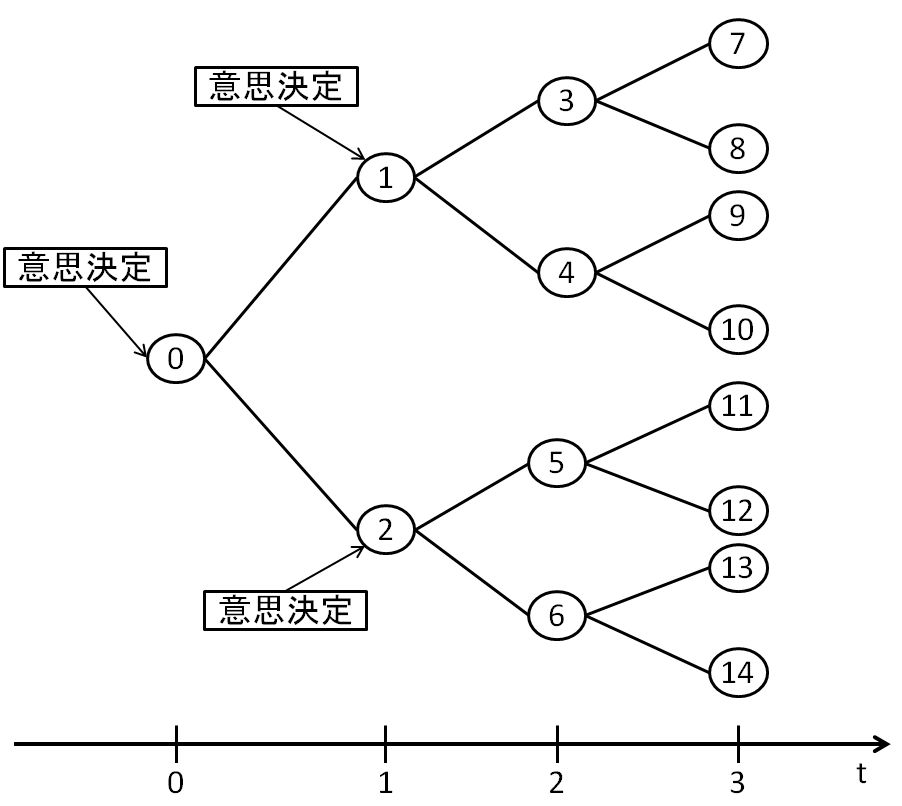
\includegraphics[width=9cm,height=7cm, clip]{tree.eps}
\caption{シナリオ・ツリー}
\label{fig:tree}
\end{figure}

本研究では,シナリオ・ツリー$t$時点での風況,蓄電池残存容量,発電出力の状態を考慮し,$t+1$時点の発電出力予測から発電計画を決定する.
未来の風況を完全に予測することは困難である.
従って,$t+1$時点の発電出力は誤差があり,$t$時点では発電出力予測が複数存在することが考えらる.
そこで本研究では,気象庁の風速データを用いて,どのようなパターンで風速が変化しているかプログラムを用いて,予測精度の確率評価を行った.

例えば,図\ref{fig:kakuritsu1},図\ref{fig:kakuritsu2}のように,風速データを2分岐(クラス)で風速$0$~$5$(m/s),$5$~(m/s)に分けて,
2期分のシナリオを作成する.
全体のシナリオの中で,それぞれのシナリオが発生すると予測される生起確率を求める.
このシナリオ・ツリーに使用する風速データは,気象庁2010年度の青森県むつ市の風速データを用いている.
青森県むつ市の風速データを使用したのは,実際に風力発電設備が設置されているためである.

\begin{figure}[h]
 \begin{minipage}{0.5\hsize}
  \begin{center}
  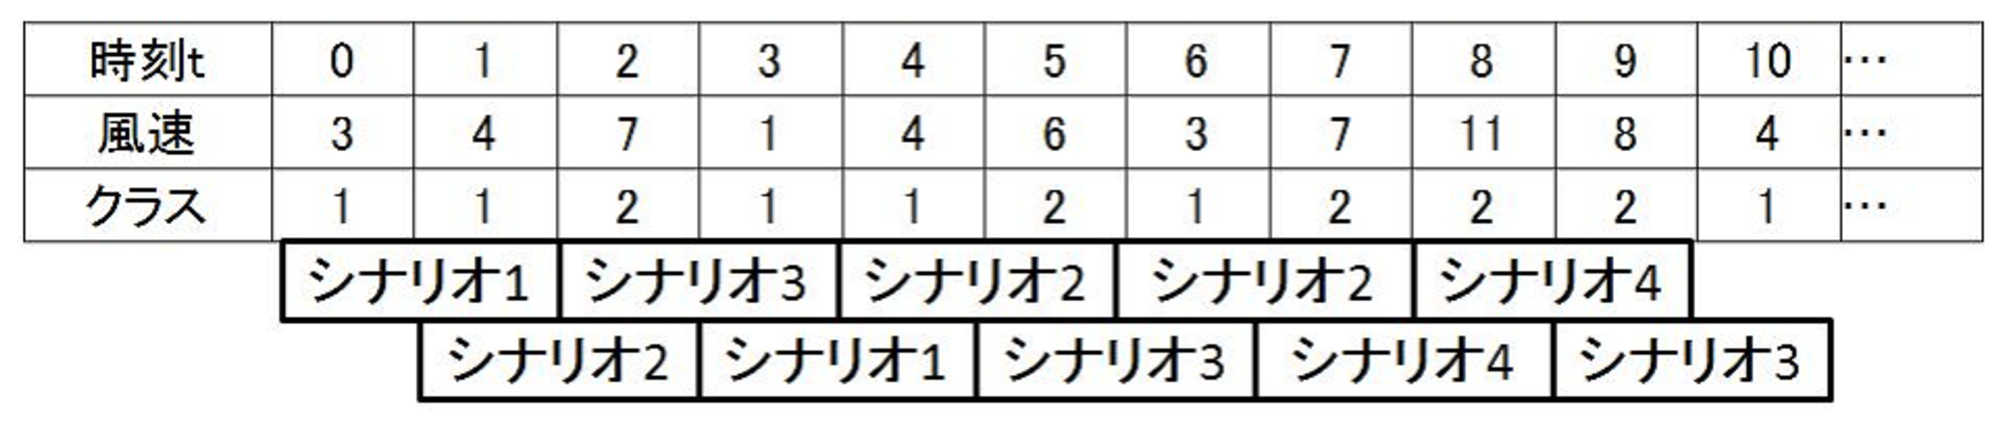
\includegraphics[width=8.5cm,height=3.5cm, clip]{kakuritsu1.eps}
  \end{center}
  \caption{シナリオ作成例}
  \label{fig:kakuritsu1}
 \end{minipage}
 \begin{minipage}{0.5\hsize}
  \begin{center}
  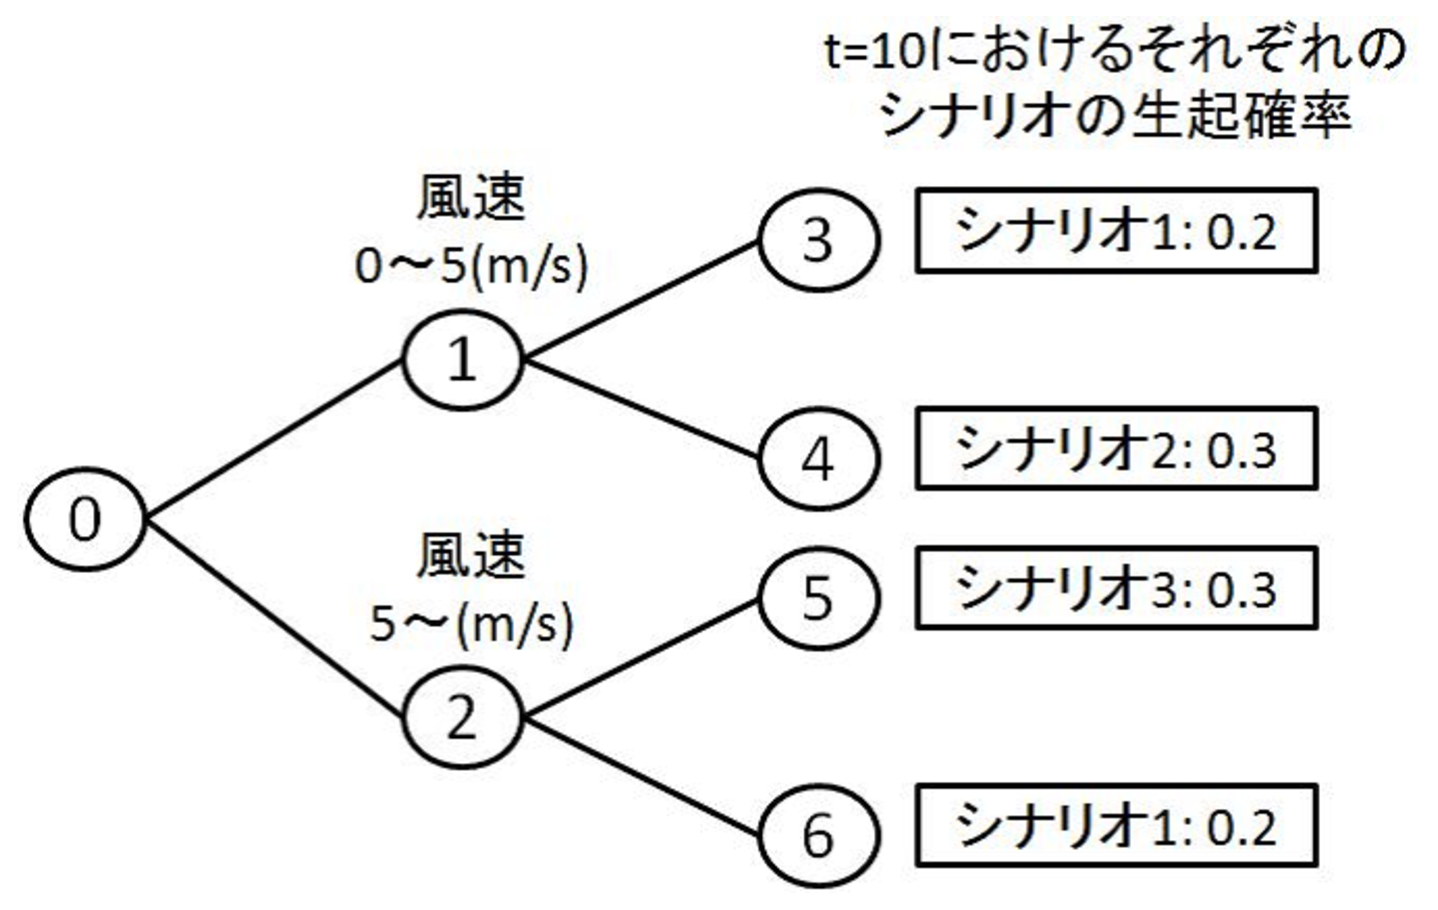
\includegraphics[width=7cm,height=6cm, clip]{kakuritsu2.eps}
  \end{center}
  \caption{生起確率作成例}
  \label{fig:kakuritsu2}
 \end{minipage}
\end{figure}

\section{最適化モデルに必要な要素}
ここでは運用計画の最適化モデルに必要な記号について説明する.

\begin{itemize}
\item 集合・添字

\begin{itemize}
\item $t \in T$: 時刻を表す添字 $t$ とその集合 $T$
\item $s \in S$: シナリオを表す添字 $s$ とその集合 $S$
\end{itemize}

\item パラメータ
\begin{itemize}
\item $\tilde{s}_{ts}$: 時刻$t$におけるシナリオ$s$に対応する,時刻$t-1$におけるシナリオ番号

\begin{figure}[h]
\centering
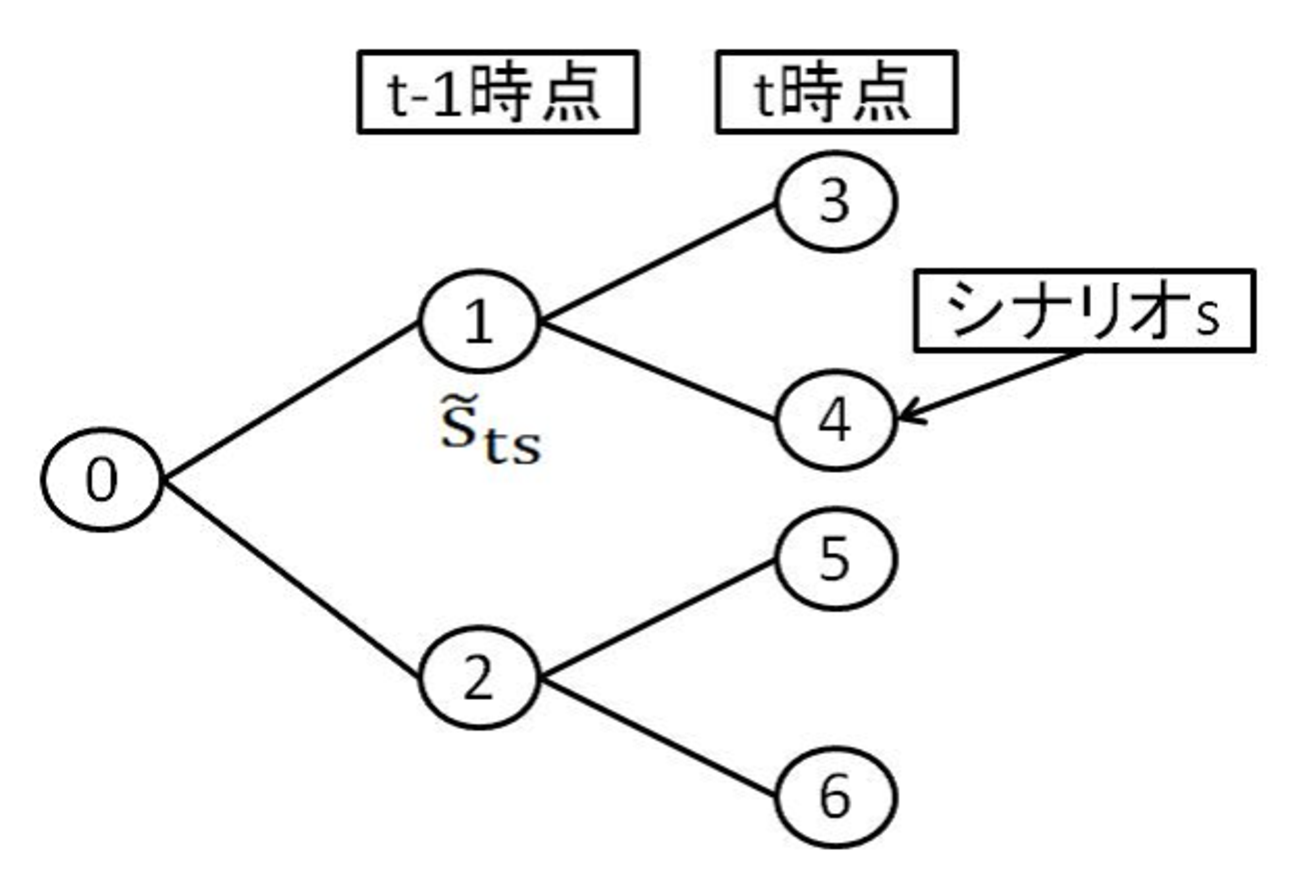
\includegraphics[width=9cm,height=5.5cm, clip]{henka.eps}
\caption{シナリオ$\tilde{s}_{ts}$に対応するシナリオ$s$}
\label{fig:henka}
\end{figure}

\item $r_t$: 時刻$t$における売電価格
\item $P_{ts}$: 時刻$t$におけるシナリオ$s$の発生確率
\item $w_{ts}$: 時刻$t$におけるシナリオ$s$での発電量
\item $CA$: 蓄電池容量
\item $\tilde{P}_U, \tilde{P}_L$: 風力発電設備の運用が破綻する確率の許容値.
$\tilde{P}_U$ は,蓄電量が,蓄電池容量のマージンを上回るシナリオの発生確率の許容値.
$\tilde{P}_L$は,マージンを下回るシナリオの発生確率の許容値.
\item $\tilde{C}_U, \tilde{C}_L$: 最終時刻における蓄電量の期待値の上下限
\item $H$: 蓄電池を作動温域になるためのヒータ損失(ヒータ損失は使用する蓄電池容量の$4$\%の電力消費を想定する)
\item $m$: マージン係数(蓄電池容量管理を行う際,完全放電や満充電状態にならないための余裕)
\item $M$: 非常に大きな正の定数(いわゆる big-M として利用する)
\end{itemize}
\item 変数
\begin{itemize}
\item $WB_t$: 時刻 $t$ において,WF(ウィンドファーム)で発電した電気のうち,蓄電池に蓄電される電気量の期待値
\item $WG_t$: 時刻 $t$ において,WF(ウィンドファーム)で発電した電気のうち,電力購入会社へ売電される電気量の期待値
\item $BG_t$: 時刻 $t$ において,蓄電池にある電気のうち,電力購入会社へ売電される電気量の期待値
\begin{itemize}
\item $WG_t + BG_t$: 時刻 $t$ において電力購入会社へ売電される電気量の期待値(= 電力購入会社への売電通告量)
\end{itemize}
\item $C_{ts}$: 時刻 $t$ におけるシナリオ $s$ においての蓄電量
\item $\delta^{1U}_{ts}, \delta^{1L}_{ts}, \delta^{2U}_{ts}, \delta^{2L}_{ts}$: 中間変数($0\mathchar`-1$ 変数)
\item $v^U_{ts}, v^L_{ts}$: 中間変数
\end{itemize}
\end{itemize}

\begin{figure}[h]
\centering
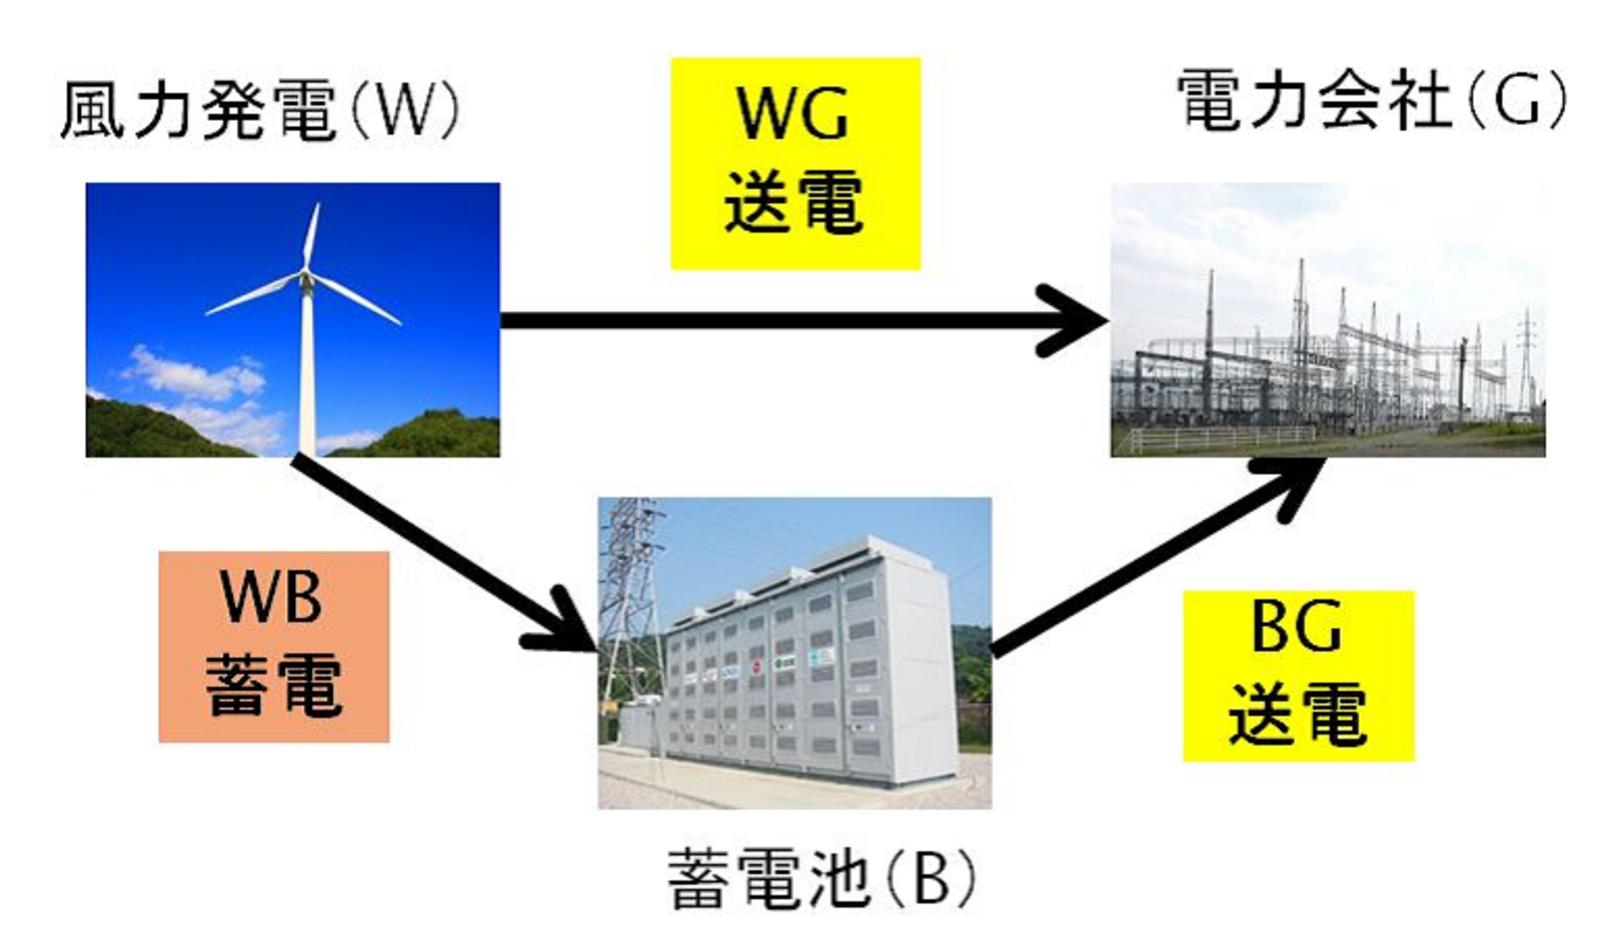
\includegraphics[width=10cm,height=6cm, clip]{WBG.eps}
\caption{風力発電の電力フロー図}
\label{fig:WBG}
\end{figure}

\section{モデルの目的関数・制約条件}

ここでは,提案する数理計画モデルの目的関数と制約条件について説明する.

【目的関数】

本モデルの目的は,(本節で示す制約条件の下で)電力の売上高を最大化することである.
電力の売上高は,次式のように書くことができる.

\begin{eqnarray}
\sum_{t = 1}^n r_t \cdot (WG_t + BG_t)
\label{eq:obuj}
\end{eqnarray}

WFの発電量と蓄電池からの放電による合成出力を電力購入会社に送電し,その時間帯の売電価格分($r_t$)の売上が見込める.

【制約条件】

\begin{eqnarray}
WB_t + WG_t = \sum_{s \in S} P_{ts} w_{ts}
\label{eq:con1}
\end{eqnarray}

時刻 $t$ におけるWFの発電量の期待値を示している.
WFで発電された電力は,電力購入会社へ送電され,発電量が計画値より過剰だった場合,その分蓄電池に送電するようになっている.

\begin{eqnarray}
&& - M (1 - \delta^{1L}_{ts})  \le 0.98 (WG_t + BG_t) - w_{ts}  \le M \delta^{1L}_{ts}
\label{eq:con2} \\
&& v^L_{ts} - M (1 - \delta^{1L}_{ts}) \le 0.98 (WG_t + BG_t) - w_{ts} \le v^L_{ts} + M (1 - \delta^{1L}_{ts})
\label{eq:con3} \\
&& - M \delta^{1L}_{ts} \le v^L_{ts} \le M \delta^{1L}_{ts}
\label{eq:con4}
\end{eqnarray}


出力一定制御型の技術要件を表している$(WG_t + BG_t)$は,送電するWFの発電量と蓄電池の送電の合成出力で,時刻$t$における計画値を表している.

(\ref{eq:con2}),(\ref{eq:con3}),(\ref{eq:con4})式は,$\delta^{1L}_{ts}$$=0$の場合と$\delta^{1L}_{ts}$$=1$の場合で
異なる意味を持つ.以下,それについて説明する.

\begin{itemize}
\item $\delta^{1L}_{ts}$$=0$の場合
\end{itemize}

(\ref{eq:con2})式は,$-M \le 0.98 (WG_t + BG_t) - w_{ts} \le 0$という式になる.
Mは十分大きな正の定数であるので,最初の不等号については事実上意味をもたない.

また,二番目の不等式では,$t$時点での実際の発電量が,(通告した計画値 - $2\%$)より多いことを示している.

また(\ref{eq:con3})式は,$-M \le 0.98 (WG_t + BG_t) - w_{ts} \le M$という式になる.
Mは十分大きな正の定数であるから,この式は事実上意味をもたない.

(\ref{eq:con4})式は,$0 \le v^L_{ts} \le 0$なので,変数$v^L_{ts}$が$0$に固定される.

\begin{itemize}
\item $\delta^{1L}_{ts}$$=1$の場合
\end{itemize}

(\ref{eq:con2})式は,$0 \le 0.98 (WG_t + BG_t) - w_{ts}\le M$という式になる.
最初の不等式では,$t$時点での実際の発電量が,(通告した計画値 - $2\%$)より少ないことを示している.

また,Mは十分大きな正の定数であるので,二番目の不等号については事実上意味をもたない.

(\ref{eq:con3})式は, $v^L_{ts} \le 0.98 (WG_t + BG_t) - w_{ts} \le v^L_{ts}$ という式になり,
$0.98 (WG_t + BG_t) - w_{ts} = v^L_{ts}$に固定される.

(\ref{eq:con4})式は,$-M \le v^L_{ts} \le M$という式になる.
Mは十分大きな正の定数であるから,この式は事実上意味を持たない.

つまり,$\delta^{1L}_{ts}$$=0$の場合は,実際の発電量が計画値の$-2$\%より多いので蓄電池からは送電せず,
$\delta^{1L}_{ts}$$=1$の場合は,実際の発電量が計画値の$-2$\%より$v^L_{ts}$の電力量が不足しているので蓄電池から送電するという制約式となっている.

\begin{eqnarray}
&& - M (1 - \delta^{1U}_{ts}) \le w_{ts} - 1.02 (WG_t + BG_t) \le M \delta^{1U}_{ts}
\label{eq:con5} \\
&& v^U_{ts} - M (1 - \delta^{1U}_{ts}) \le w_{ts} - 1.02 (WG_t + BG_t) \le v^U_{ts} + M (1 - \delta^{1U}_{ts})
\label{eq:con6} \\
&& - M \delta^{1U}_{ts} \le v^U_{ts} \le M \delta^{1U}_{ts}
\label{eq:con7}
\end{eqnarray}

出力一定制御型の技術要件を表している$(WG_t + BG_t)$は,送電するWFの発電量と蓄電池の送電の合成出力で,
時刻$t$における計画値を表している.

(\ref{eq:con5}),(\ref{eq:con6}),(\ref{eq:con7})式は,$\delta^{1L}_{ts}$$=0$の場合と$\delta^{1L}_{ts}$$=1$の場合で
異なる意味を持つ.以下,それについて説明する.

\begin{itemize}
\item $\delta^{1L}_{ts}$$=0$の場合
\end{itemize}

(\ref{eq:con5})式は,$-M \le w_{ts} - 1.02 (WG_t + BG_t)\le 0$という式になる.
Mは十分大きな正の定数であるので,最初の不等号については事実上意味をもたない.

また,二番目の不等式では,$t$時点での実際の発電量が,(通告した計画値 + $2\%$)より少ないことを示している.

(\ref{eq:con6})式は,$-M \le w_{ts} - 1.02(WG_t + BG_t) \le M$という式になる.
Mは十分大きな正の定数であるから,この式は事実上意味を持たない.

(\ref{eq:con7})式は,$0 \le v^L_{ts} \le 0$という式になるので,変数$v^L_{ts}$は$0$に固定される.

\begin{itemize}
\item $\delta^{1L}_{ts}$$=1$の場合
\end{itemize}

(\ref{eq:con5})式は,$0 \le w_{ts} - 1.02 (WG_t + BG_t)\le M$という式になる.
最初の不等式では,$t$時点での実際の発電量が,(通告した計画値 + $2\%$)より多いことを示している.

また,Mは十分大きな正の定数であるので,二番目の不等号については事実上意味をもたない.

(\ref{eq:con6})式は,$v^L_{ts} \le w_{ts} - 1.02(WG_t + BG_t) \le v^L_{ts}$という式となり,
$w_{ts} - 1.02(WG_t + BG_t) = v^L_{ts}$に固定される.

(\ref{eq:con7})式は,$-M \le v^L_{ts} \le M$という式になる.
Mは十分大きな正の定数であるから,この式は事実上意味を持たない.

つまり,$\delta^{1L}_{ts}$$=0$の場合は,実際の発電量が計画値の$+2$\%より少ないので蓄電池からは送電せず,
$\delta^{1L}_{ts}$$=1$の場合は,実際の発電量が計画値の$+2$\%より多いので蓄電池へ充電するという制約式となっている.



\begin{eqnarray}
C_{ts} = C_{t-1,\tilde{s}_{ts}} - \frac{1}{0.9} v^L_{ts} + 0.95 v^U_{ts} - H
\label{eq:con8}
\end{eqnarray}

シナリオ$\tilde{s}_{ts}$から,時刻$t$におけるシナリオ$s$への蓄電池の変化量を表している.

時刻$t-1$から時刻$t$における蓄電量の変化において充電と放電を同時に行うことはありえない.
よって,$v^L_{ts} \ge 0$である場合は,$v^U_{ts} = 0$であり,
$v^U_{ts} \ge 0$である場合は,$v^L_{ts} = 0$である.

シナリオ$s$に対応するシナリオ$\tilde{s}_{ts}$は図\ref{fig:henka}のようになっている.



\begin{figure}[h]
\centering
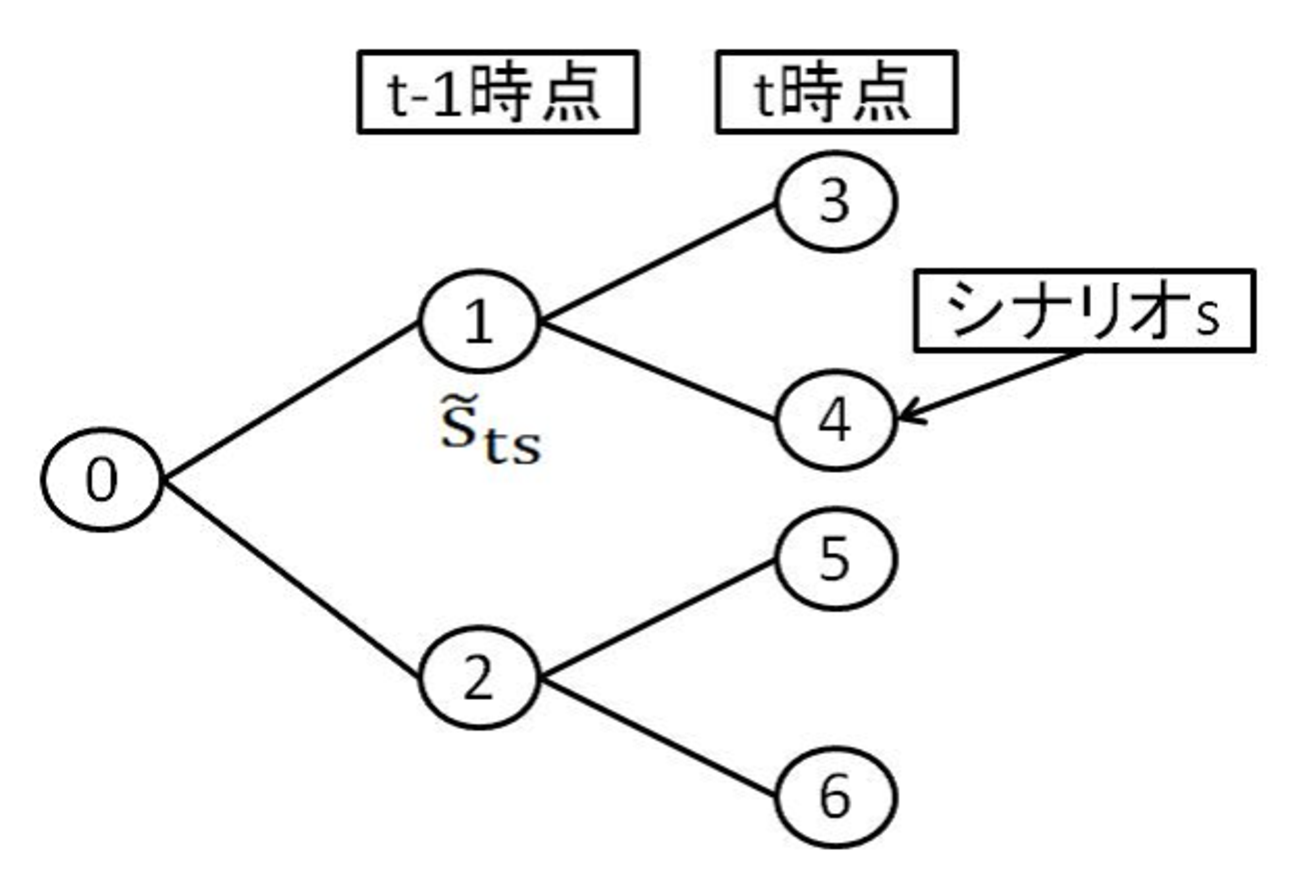
\includegraphics[width=9cm,height=5.5cm, clip]{henka.eps}
\caption{シナリオ$\tilde{s}_{ts}$に対応するシナリオ$s$}
\label{fig:henka}
\end{figure}

WFから直接電力系統に送電する際はロスなく送電できるが,蓄電池を経由して電力系統に送電する場合は充放電効率によるロスと
蓄電池を作動温域にするためのヒータ損失を考慮しなくてはならない.
蓄電池を経由する際のロスとヒータ損失を図\ref{fig:loss}に示す.

\begin{figure}[h]
\centering
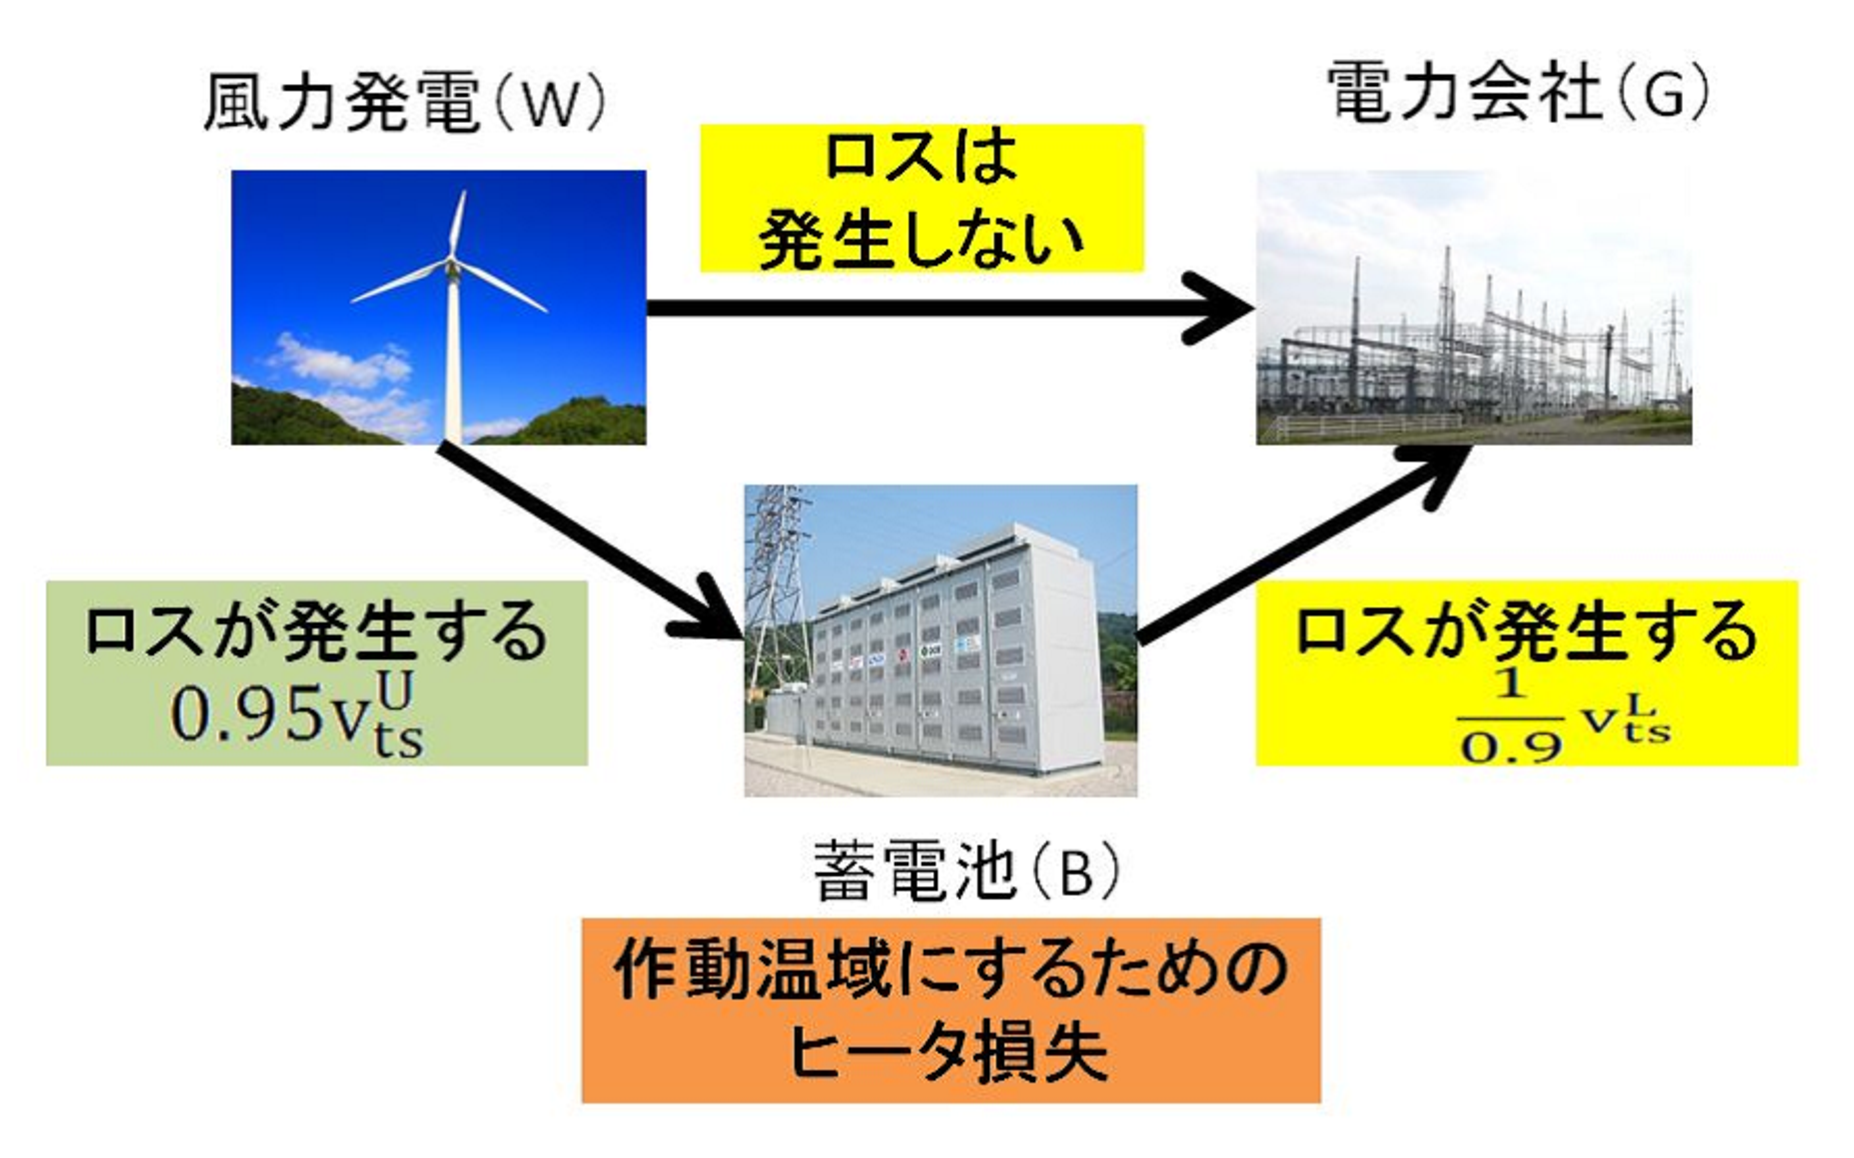
\includegraphics[width=9cm,height=7cm, clip]{loss.eps}
\caption{充放電に関係する電力損失}
\label{fig:loss}
\end{figure}

\begin{eqnarray}
&& - M (1 - \delta^{2L}_{ts}) \le m * CA - C_{ts} \le M \delta^{2L}_{ts}
\label{eq:con9} \\
&& - M (1 - \delta^{2U}_{ts}) \le C_{ts} - m * CA \le M \delta^{2U}_{ts}
\label{eq:con10}
\end{eqnarray}

蓄電池容量の確保するマージンを表しており,確保したマージン以内に蓄電量が収まるように調整する.
$m$は,確保するマージンの係数を表しており,蓄電池のマージンを上下限$m * CA$の容量で確保するようにしている.

(\ref{eq:con9}),(\ref{eq:con10})式は,$\delta^{1L}_{ts}$$=0$の場合と$\delta^{1L}_{ts}$$=1$の場合で
異なる意味を持つ.以下,それについて説明する.

\vspace{\Cvs}
(\ref{eq:con9})式は,時刻$t$における蓄電量がマージンの下限を下回っていないかを表す制約式である.

\begin{itemize}
\item $\delta^{2L}_{ts}$$=0$の場合
\end{itemize}

$-M \le m * CA - C_{ts}\le 0$という式となる.
Mは十分大きな正の定数であるので,最初の不等号については事実上意味をもたない.

また,二番目の不等式では,$t$時点での蓄電量が,マージンの下限より多いことを示している.

\begin{itemize}
\item $\delta^{2L}_{ts}$$=1$の場合
\end{itemize}

$0 \le m * CA - C_{ts}\le M$という式となる.
最初の不等式では,$t$時点での蓄電量が,マージンの下限より少ないことを示している.

また,Mは十分大きな正の定数であるので,二番目の不等号については事実上意味をもたない.

\vspace{\Cvs}
(\ref{eq:con10})式は,時刻$t$における蓄電量がマージンの上限を上回っていないかを表す制約式である.

\begin{itemize}
\item $\delta^{2U}_{ts}$$=0$の場合
\end{itemize}

$-M \le C_{ts} - m * CA \le 0$という式となる.
Mは十分大きな正の定数であるので,最初の不等号については事実上意味をもたない.

また,二番目の不等式では,$t$時点での蓄電量が,マージンの上限より少ないことを示している.

\begin{itemize}
\item $\delta^{2U}_{ts}$$=1$の場合
\end{itemize}
$0 \le C_{ts} - m * CA\le M$という式となる.
最初の不等式では,$t$時点での蓄電量が,マージンの上限より多いことを示している.

また,Mは十分大きな正の定数であるので,二番目の不等号については事実上意味をもたない.


\begin{eqnarray}
&& \sum_{s \in S} \delta^{2L}_{ts} P_{ts} \le \tilde{P}_L
\label{eq:con11} \\
&& \sum_{s \in S} \delta^{2U}_{ts} P_{ts} \le \tilde{P}_U
\label{eq:con12}
\end{eqnarray}

(\ref{eq:con11})式は,時刻$t$における(\ref{eq:con9})式で$\delta^{2L}_{ts}$が$1$の場合であり,
容量管理が出来ていないシナリオ$s$の発生確率の総和が,蓄電池のマージンの上限を上回る発生確率の許容値を,
超えないようにしている.

(\ref{eq:con12})式は,時刻$t$における(\ref{eq:con10})式で$\delta^{2U}_{ts}$で$1$の場合であり,
容量管理が出来ていないシナリオ$s$の発生確率の総和が,蓄電池のマージンの下限を下回る発生確率の許容値を,
超えないようにしている.

\begin{eqnarray}
\tilde{C}_L \le \sum_{s \in S} C_{ns} \le \tilde{C}_U
\label{eq:con13}
\end{eqnarray}

最終時刻における蓄電量の期待値の上下限以内に,最終時刻の蓄電量が収まるようにする.

%\chapter{数値実験}
%本節では,運用計画モデルの数値実験の説明と実験結果および考察を行う.
%\section{実験内容}
%ここでは,提案した運用計画モデルが有用であるかどうかを調べるために行った数値実験について説明する.
%発電計画の通告時間,通告更新周期は2時間とした.
%シナリオ・ツリーのクラス(分岐)数,期間数を変え,様々なシナリオの発生確率を求める.
%クラス(分岐)数と期間数の数を増やすとそれぞれのシナリオの生起確率の精度が上がるので,そのシナリオでの発電量の発生確率の精度も上がる.
%またシナリオの生起確率から計画破綻の許容確率を設定する.
%蓄電池容量をWFの定格出力の40\%から100\%の間で設定し,マージンを上下限5\%~30\%の間で設定する.
%それぞれの期間で売電価格を昼間なら9~11(円/kWh),夜間なら7~9(円/kWh)として設定する.
%本実験は,シナリオ・ツリーの分岐数,期間数,売電価格,計画破綻の発生許容確率のパラメータを決定し,
%それに基づき蓄電池容量とマージンの上下限を変えて,複数のパターンで実験を行う.
%\section{実験結果,考察}
%数値実験の結果は,以下のようになった.

\chapter{数値実験}

本章では,前章で提案した運用計画モデルを用いた数値実験の説明を行う.

\section{実験内容}

ここでは,本研究で行った数値実験の内容について説明する.

まず,本実験では,発電計画の通告時間,ならびに通告更新周期を $2$ 時間と設定した.
これは,風力発電設備が売電するときの標準的な設定である\cite{電力}.

また,本実験では,シナリオ・ツリーの分岐数と期間数を変え,実験を行う.
分岐数と期間数の設定は,本実験において重要な意味を持つ.
なぜなら,シナリオ・ツリーの葉の数,すなわち最終期におけるシナリオの数は,「(分岐数)の(期間数)乗」となる.
この量に支配される変数や制約の数が存在するため,分岐数や期間数を大きく設定しすぎると,
実用上意味のある時間では最適解を求めることが出来なくなる可能性がある.

本実験では,表\ref{tb:1}にあるような分岐数・計画期間数の下で実験を行った.
%
\begin{table}[h]
\begin{center}
  \caption{本実験における分岐数・計画期間数の設定}
  \label{tb:1}
  \begin{tabular}{|r|r|}
  \hline
  分岐数 & 期間数 \\
  \hline
  \hline
  2 & 3 \\
  \hline
  2 & 4 \\
  \hline
  2 & 5 \\
  \hline
  2 & 6 \\
  \hline
  3 & 3 \\
  \hline
  3 & 4 \\
  \hline
  4 & 3 \\
  \hline
  4 & 4 \\
  \hline
  \end{tabular}
\end{center}
\end{table}
%

表 \ref{tb:1} にある設定の下で実験を行ったのは,予備実験の結果,これ以上の問題規模に対しては,
現実的な時間で問題の最適解を得ることが難しいと考えられるからである.
ここでいう「現実的な時間」とは,上で述べた,発電計画の通告時間ならびに通告更新周期の $2$ 時間を指す.
$2$ 時間毎に計画を買い取り側に通告する必要があることから,最適化計算はこれ以上の時間を要してはならない.

今回の数値実験では,青森県むつ市にある,むつ小川原ウィンドファームの発電所を想定し
て行った(http://www.eco-power.co.jp/hatudensho/17\_mutu.html).
この発電所には,定格出力1500(kW)の発電機が $21$ 機設置されている.
本実験中で用いる風力発電所に固有の値は,全てこの発電所と同じ値を用いることとした.

また,各シナリオの生起確率は,第\ref{model}章で述べたように,気象庁による青森県むつ市の風速データを用いて算出した.
さらに,計画期間中の予測値は,いずれも $5.0$ (m/s) であるものと仮定して実験を行った.
ただし,本研究の主たるテーマでもあるように,この予測値はあくまで予測であり,実際の値ではない.
そこで,実際の風速は,この予測値から $15$ \% の変動幅内で一様に発生するものとした.
なお,変動幅 $15$ \% であるという仮定は,予測値と実測値とを比較した過去の研究\cite{徳谷}に基づいている.
そして,その変動幅を(後に示す)分岐数で均等分割することで,一つのシナリオを形成するようにした.
また,売電価格は,昼間の売電価格として標準的な $10$ (円/kWh) と設定した.

さらに,表 \ref{tb:1} に示した分岐数・計画期間数に対して実験を行う際に,
蓄電池容量に対するマージン係数 $m$ と,蓄電池容量 $CA$ を変動させている.
$m$ については $0.05$(蓄電池容量の $5$ \% から $95$ \% の範囲を利用可能)
から $0.30$(蓄電池容量の $30$ \% から $70$ \% の範囲を利用可能)まで$0.05$ 刻みで設定した.
また $CA$ については,WF の定格容量に対する蓄電池容量の比として,$0.3$ から $1.0$ の $0.1$ 刻みで実験を行った.

本実験で用いた計算機環境・ソフトウェアは以下の通りである.
%
\begin{table}[h]
\begin{center}
  \begin{tabular}{|l|l|}
  \hline
  計算機 & Dell XPS 8300 \\
  (OS) & Windows 7 Professional SP1 \\
  (CPU) & Inter(R) Core(TM) i7-2600 CPU @ 3.40GHz \\
  (RAM) & 16.0 GB \\
  \hline
  ソルバ & SCIP version 2.1.1 \\
  \hline
  \end{tabular}
\end{center}
\end{table}
%

用いている計算機は,標準的なデスクトップパソコンであると言える.また最適化問題を解くために,
SCIP \cite{SCIP}というソルバを用いた.
SCIP はアカデミック・フリーのソルバの中では世界的に最も早いソルバの一つである.
今回は,第\ref{model}章で提案した最適化モデルを
AMPL\cite{AMPL}と呼ばれるモデリング言語で記述し,
それを glpk\cite{GLPK}というソフトウェアで SCIP 可読な .lp 形式のファイルに変換することで,
SCIP を利用した.

\section{実験結果}

ここでは,前節で説明した設定の下で行った数値実験の結果を示す.

各分岐数と期間数毎による蓄電池容量とマージン設定の違いによる売電収入の図\ref{fig:C2_T3}~図\ref{fig:C4_T4}とそれにかかった計算時間の平均と分散の表\ref{tb:2}を記す.



%\begin{itemize}
%\item memo: 掲載するべき図等
     % \begin{itemize}
    %\item margin, ratio と利益のグラフ(各分岐数・期間数毎)
    %\item 計算時間(平均,分散)(表で)
      %\end{itemize}
%\end{itemize}

\begin{figure}[]
 \begin{minipage}{0.5\hsize}
  \begin{center}
   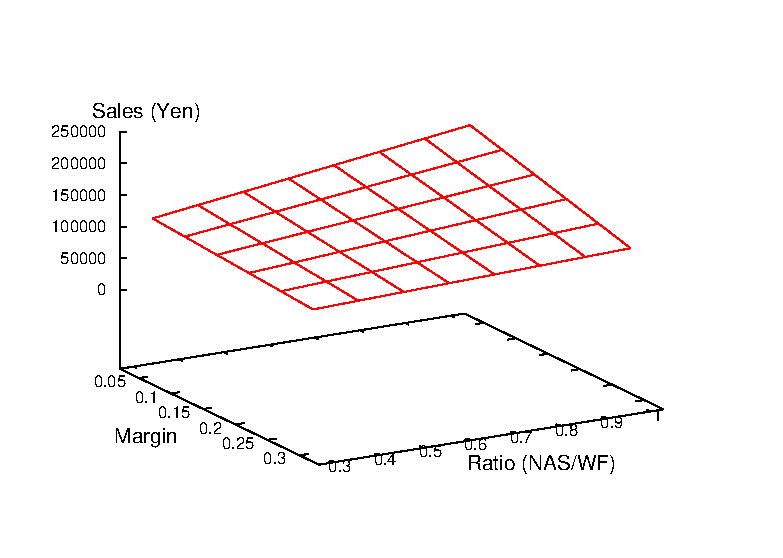
\includegraphics[width=10cm,height=8cm, clip]{stdout_C2_T3_data_m.eps}
  \end{center}
  \caption{2分岐,3期間の場合}
  \label{fig:C2_T3}
 \end{minipage}
 \begin{minipage}{0.5\hsize}
  \begin{center}
   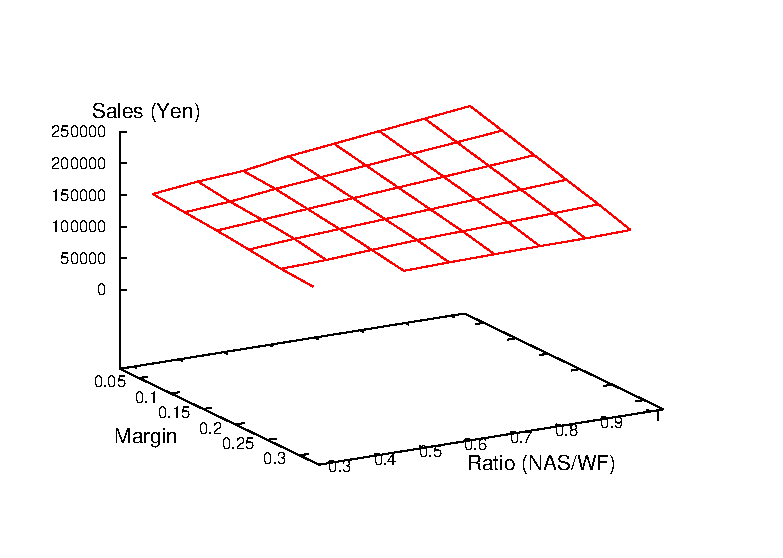
\includegraphics[width=10cm,height=8cm, clip]{stdout_C2_T4_data_m.eps}
  \end{center}
  \caption{2分岐,4期間の場合}
  \label{fig:C2_T4}
 \end{minipage}
\end{figure}

\begin{figure}[]
 \begin{minipage}{0.5\hsize}
  \begin{center}
   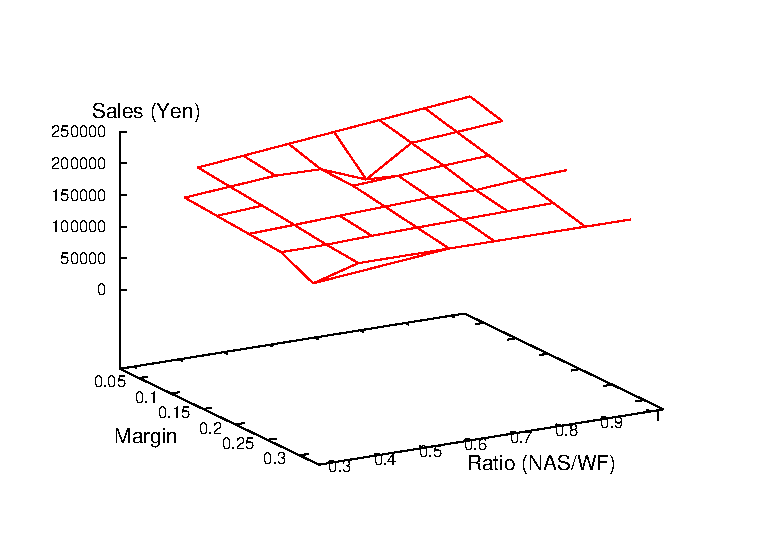
\includegraphics[width=10cm,height=8cm, clip]{stdout_C2_T5_data_m.eps}
  \end{center}
  \caption{2分岐,5期間の場合}
  \label{fig:C2_T5}
 \end{minipage}
 \begin{minipage}{0.5\hsize}
  \begin{center}
   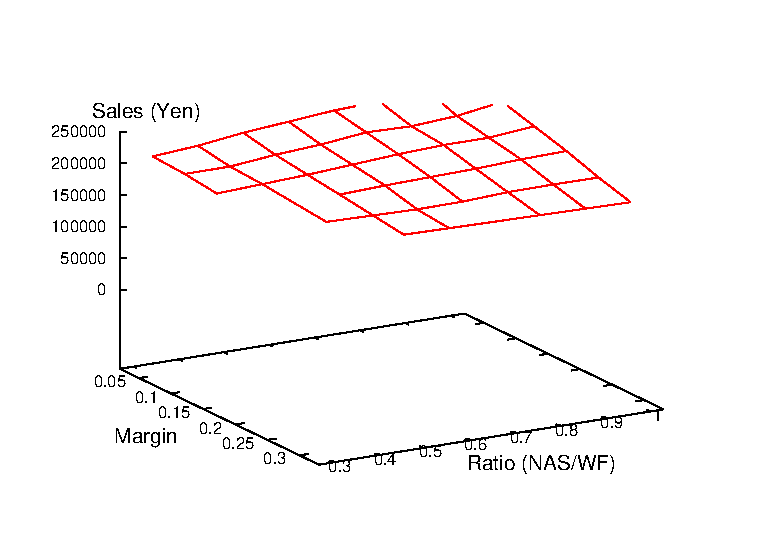
\includegraphics[width=10cm,height=8cm, clip]{stdout_C2_T6_data_m.eps}
  \end{center}
  \caption{2分岐,6期間の場合}
  \label{fig:C2_T6}
 \end{minipage}
\end{figure}

\begin{figure}[]
 \begin{minipage}{0.5\hsize}
  \begin{center}
   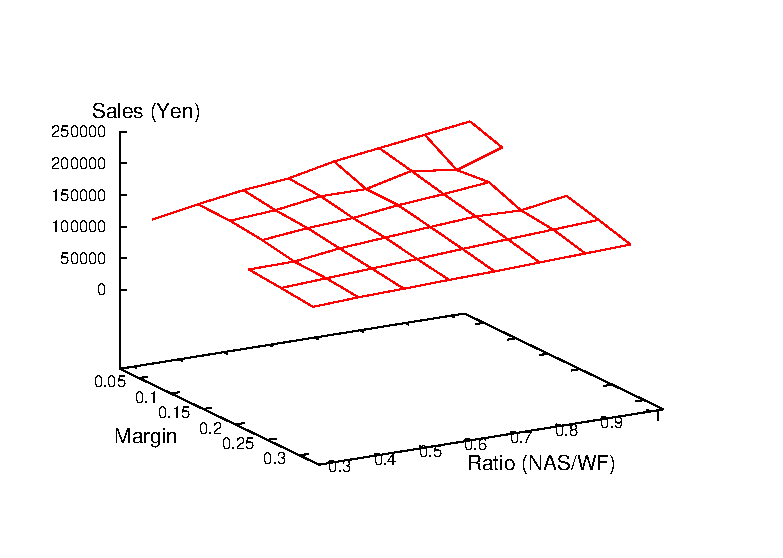
\includegraphics[width=10cm,height=8cm, clip]{stdout_C3_T3_data_m.eps}
  \end{center}
  \caption{3分岐,3期間の場合}
  \label{fig:C3_T3}
 \end{minipage}
 \begin{minipage}{0.5\hsize}
  \begin{center}
   \includegraphics[width=10cm,height=8cm, clip]{stdout_C3_T4_data_m.eps}
  \end{center}
   \caption{3分岐,4期間の場合}
  \label{fig:C3_T4}
 \end{minipage}
\end{figure}

\begin{figure}[]
 \begin{minipage}{0.5\hsize}
  \begin{center}
   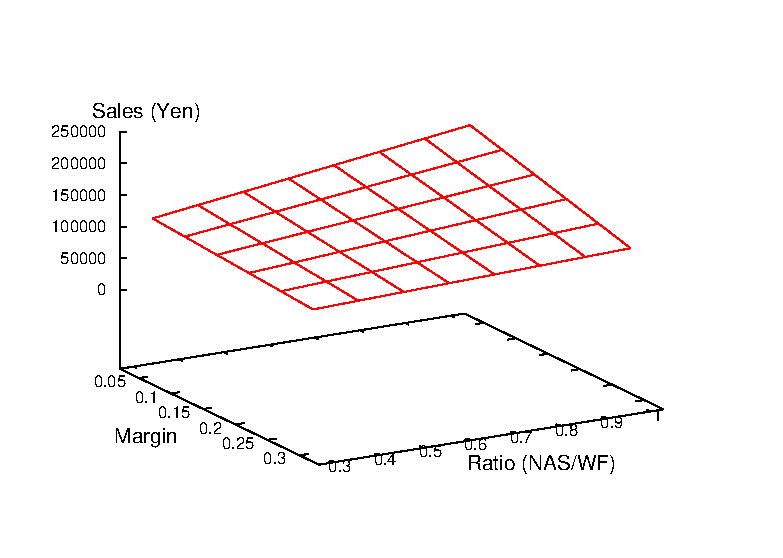
\includegraphics[width=10cm,height=8cm, clip]{stdout_C4_T3_data_m.eps}
  \end{center}
  \caption{4分岐,3期間の場合}
  \label{fig:C4_T3}
 \end{minipage}
 \begin{minipage}{0.5\hsize}
  \begin{center}
   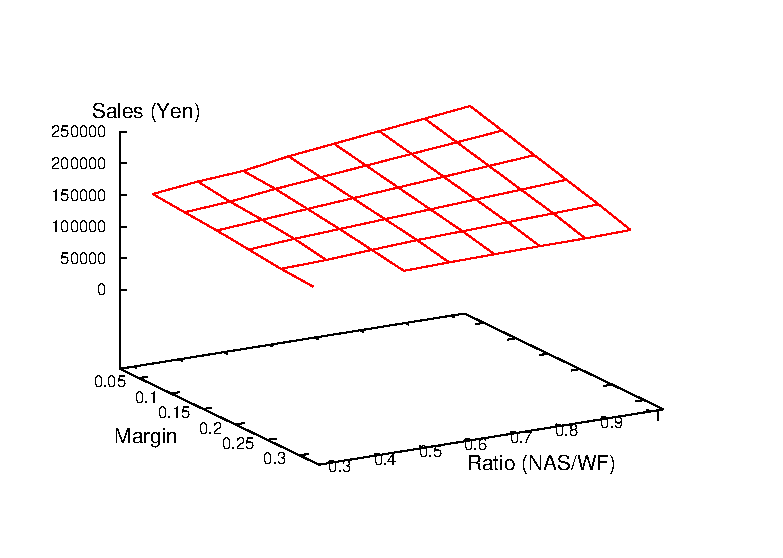
\includegraphics[width=10cm,height=8cm, clip]{stdout_C4_T4_data_m.eps}
  \end{center}
  \caption{4分岐,4期間の場合}
  \label{fig:C4_T4}
 \end{minipage}
\end{figure}

\newpage
\begin{table}[]
\begin{center}
  \caption{本実験における計算時間(s)の平均・分散}
  \label{tb:2}
  \begin{tabular}{|c|c|c|c|c|c|c|c|c|}
  \hline
  分岐数・期間数 & 2・3 & 2・4 & 2・5 & 2・6 & 3・3 & 3・4 & 4・3 & 4・4 \\
  \hline
  平均 & 0.34 & 8.45 & 192.94 & 1244.24 & 120.70 & 0.36 & 8.66 & 201.18 \\
  \hline
  分散 & 0.10 & 4.60 & 271.61 & 1211.01 & 96.50 & 0.16 & 4.73 & 283.39 \\
  \hline
  %&分岐数4期間数5 & 0.34 & 0.10\\
  %\hline
  \end{tabular}
\end{center}
\end{table}

図\ref{fig:C2_T3}~図\ref{fig:C4_T4}で線が描かれていない場所は,最適解が得られなかったものである.
結果から見ると,分岐数や期間数が多くなっていくと最適解を得られないことが多くなった.
またマージン係数と蓄電池容量は,それぞれの最小値と最大値に近づくと最適解を得られにくい傾向にある.
表\ref{tb:2}における結果からは,分岐数と期間数における計算時間の増加の違いがみえる.
基本的には分岐数の増加による計算時間の平均・分散の増加は小さく,期間数の増加による計算時間の平均・分散の増加は大きい.

%\begin{figure}[]
%\centering
%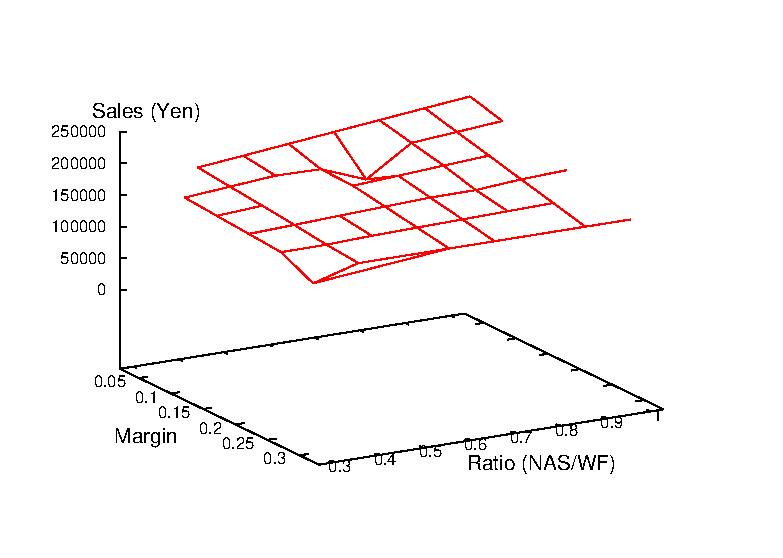
\includegraphics[width=12cm,height=6.5cm, clip]{stdout_C4_T5_data_m.eps}
%\caption{4分岐,5期間実験結果}
%\label{fig:C4_T5}
%\end{figure}


\newpage
\section{考察}
ここでは,前節で示した実験結果についての考察を行う.

まず,図\ref{fig:C2_T3}~図\ref{fig:C4_T4}に共通する傾向として,
%
\begin{quotation}
WF の定格出力に対する蓄電池容量の比が同じであれば,マージン係数が小さい
(蓄電池容量に対して利用できる範囲が大きい)方が電力の売上高が大きくなる
\end{quotation}
%
という点が挙げられる.
これは,今回の数値実験において,蓄電池のマージン制約が破綻する許容確率を,
各最適化計算において一定に定めていることによるものである.
すなわち,許容確率が一定であれば,蓄電池の使用可能領域がより大きい方が売上高が大きくなる.

一方,
%
\begin{quotation}
マージン係数が一定のとき,WF の定格出力に対する蓄電池容量の比を大きくしても,
必ずしも売上高は大きくならない
\end{quotation}
%
という現象も確認することができる.
蓄電池の容量が大きい場合,蓄電できる容量は大きくなるわけだが,逆に蓄電池の温度維持に必要となる電力も大きいため,
必ずしも利益には結びつかないということだと考えられる.
今回の実験では予測値が $5.0$ (m/s) の場合を扱っているが,予測値(あるいは平均風速)がこれよりも大きい場合は,
また違った傾向が観察されるものと考えられる.

最適化計算に要する時間については,問題によってかなりの差が観察された.
これは,ソルバが用いている解法(分枝限定法や切除平面法)の特性によるものではあるが,
本問題においては求解に用いることができる時間に限りがある(通告時間・通告更新周期を越えて計算することはできない)ため,
注意が必要である.
一つの対応としては,求解時間に制限を設けて計算を行うことであるが,その場合得られる解には厳密性の保証がない.

なお,今回の実験においては,最適化計算が正常終了しないケースが散見された.
これは,モデル作成の不備ではなく,利用したソルバの数値的エラーに関するものであることが確認できている.
今回利用したソルバはソースコードも併せて配布しているため,そのエラー発生箇所を調べることも原理的には可能な状態ではあったが,
非常に大規模なプログラムであるため,今回はその作業を断念した.
この点については,今後の課題としたい.

\chapter{おわりに}
本研究では,風力発電の運用計画をシナリオ・ツリーを用いたモデル化を行い,数値実験で各種条件を変えても
安定した運用が継続できるかを示した.
シナリオ・ツリーの確率評価に用いた,気象庁の風速データは青森県むつ市2010年の1年分のデータでしかできなかった.
さらに精度の高いシナリオの発生確率求めるには,より多くの風速データで確率評価を行う必要がある.
本研究では,出力一定制御型に対する運用計画の立案を行ったが,蓄電池併設風力発電には出力変動緩和型の制御型も提案されている.
今回は出力変動緩和型の運用計画の立案はできなかったが,こちらの安定運用の計画も立案し,出力一定制御型の運用計画との違いを
検証していくことが今後の課題と考える.

%※書き足すべきこと(文章はそのままでなくてもよいが,同じような内容を含める必要あり)

今後の課題としては,シナリオ・ツリーで扱うシナリオを絞り込むことが挙げられる.
本研究では,各時間帯において単純に定められた数の分岐を行っている.
これは,未来のシナリオは過去に起きたすべてのことに依存する,ということに他ならないが,同じような状態をまとめることが可能な場合もある.
%
本研究で扱っている対象,すなわち風向・風力をそのように扱うことの是非を検討し,もし可能であれば似た状態をまとめることで,
$1$ 期あたりの分岐数を増やしたり,考慮する期間数を増やすことが可能になる.
この可能性について検討する必要がある.


\begin{thebibliography}{17}



\bibitem{GLPK}
GLPK (GNU Linear Programming Kit)

http://www.gnu.org/software/glpk/

\bibitem{シナリオ}
枇々木 規雄,多期間ポートフォリオ最適化問題のための数理計画モデル

\bibitem{変動緩和}
星野 直樹(株)日立エンジニアリング・アンド・サービス 新エネルギー本部,出力変動緩和制御型風力発電システムのご紹介

http://http://jwpa.jp/2011\_pdf/90-09mado.pdf

\bibitem{エネルギー}
経済産業省・資源エネルギー庁,エネルギー白書2010

http://www.enecho.meti.go.jp/topics/hakusyo/2010/index.htm

\bibitem{風力}
北村清之,風力発電と蓄電池の制御技術

http://www.ueri.co.jp/jhif/WG/WG4/WG4\_01.pdf

\bibitem{設備}
水口健一,電気設備の知識と技術

http://saijiki.sakura.ne.jp/denki2/air.html

\bibitem{NEDO}
NEDO(独立行政法人新エネルギー・産業技術総合開発機構),日本における風力の状況・世界における風力発電の状況

http://www.nedo.go.jp/library/fuuryoku/index.html

\bibitem{予測}
NEDO(独立行政法人新エネルギー・産業技術総合開発機構),気象予測に基づく風力発電予測システムの開発

http://app3.infoc.nedo.go.jp/gyouji/events/FF/nedoevent.2008-03-31.8093938166/

8cc765998\_98a8529b5b895b9a5316(6c178c61PJ).pdf

\bibitem{併設}
日本風力開発株式会社,蓄電池併設型風力発電の可能性(2005)

http://www.meti.go.jp/committee/materials/downloadfiles/g50606a41j.pdf

\bibitem{AMPL}
Robert Fourer,David M. Gay,Brian W. kernighan,AMPL(A Modeling Language for Mathematical Programming)

\bibitem{SCIP}
SCIP 混合整数計画(MIP)ソルバー

http://scip.zib.de/

\bibitem{電力}
谷川亮一,青木功,田邊隆之,電力ソリューション特集

http://www.meidensha.co.jp/pages/tech/tech01/review-200903/article-200903-0051.pdf

\bibitem{出力一定}
谷川亮一(伊藤忠テクノソリューションズ),蓄電池等併設型風力発電システムでの出力一定制御方法における
風力発電出力予測方法の検討

http://http://www.engineering-eye.com/rpt/r070\_power\_and\_energy200806a/pdf/

r\_power\_and\_energy200806a.pdf

\bibitem{蓄電池}
辰巳国昭 独立行政法人産業技術総合研究所 ユビキタスエネルギー研究部門,系統安定化に向けた蓄電池技術の動向と課題

http://http://www.meti.go.jp/committee/materials2/downloadfiles/g80808a07j.pdf


\bibitem{徳谷}
徳谷祐貴,不完全情報化において風力発電を効率的に運用する計画の立案

\bibitem{牛山}
牛山泉,風力エネルギー読本

\bibitem{吉田}
吉田穣,風力発電量の試算方法についての検討

http://www.tronc.co.jp/pdfweb/evv284w.pdf

\end{thebibliography}



%
\end{document}